\documentclass[aspectratio=43]{beamer}

% ──────────────────────────────────────────────────────────────────────────────
%                         BEAMER DOCUMENT PREAMBLE
% ──────────────────────────────────────────────────────────────────────────────

% ──────────────────────────────────────────────────────────────────────────────
% 0. BASICS/UTILITY
% ──────────────────────────────────────────────────────────────────────────────
\usepackage{amsmath}
\usepackage{extarrows}
\usepackage{pgffor}
\usepackage{array}
\usepackage{graphicx}
\usepackage[svgnames]{xcolor}
\usepackage[percent]{overpic}
\usepackage[export]{adjustbox}
\usepackage{xparse}
\usepackage[backend=biber]{biblatex}
\DeclareMathOperator*{\argmax}{arg\,max}
\DeclareMathOperator*{\argmin}{arg\,min}

% ──────────────────────────────────────────────────────────────────────────────
% 1. THEME & FONT THEME
% ──────────────────────────────────────────────────────────────────────────────
\usetheme{default}                  % Base beamer theme
\usecolortheme{default}             % Base color theme
\usefonttheme{structurebold}        % Bold structural fonts

% ──────────────────────────────────────────────────────────────────────────────
% 2. PAGE MARGINS & FRAME TITLE LAYOUT
% ──────────────────────────────────────────────────────────────────────────────
\setbeamersize{text margin left=1.5cm, text margin right=1.5cm}
\setbeamertemplate{frametitle}[default][%
  left,                              % Align title to the left
  leftskip=0.5cm,                    % Indent from left edge
  sep=0.5cm                          % Space between title and content
]

% ──────────────────────────────────────────────────────────────────────────────
% 3. COLOR DEFINITIONS
% ──────────────────────────────────────────────────────────────────────────────
\definecolor{primaryblue}{RGB}{70, 130, 180}  % Accent blue
\definecolor{primaryred}{RGB}{229, 57, 53}  % Accent red
\definecolor{lightgray}{RGB}{245, 245, 245}   % Light background gray
\definecolor{darkgray}{RGB}{80, 80, 80}       % Dark text gray
\definecolor{bluegrey}{RGB}{120, 144, 156}     % Caption label color
\definecolor{grey}{RGB}{158, 158, 158}          % Caption text color
\definecolor{cquoteframe}{RGB}{30,60,100}          % Quote box frame
\definecolor{cquoteback}{RGB}{240,245,252}          % Quote box background fill

% ──────────────────────────────────────────────────────────────────────────────
% 4. BEAMER COLOR THEMES
% ──────────────────────────────────────────────────────────────────────────────
\setbeamercolor{structure}{fg=primaryblue}    % Structural elements
\setbeamercolor{frametitle}{fg=primaryblue}   % Frame title

% Block styles
\setbeamercolor{block title}{bg=primaryblue, fg=white}
\setbeamercolor{block body}{bg=lightgray}
\setbeamercolor{block title alerted}{bg=red!80, fg=white}
\setbeamercolor{block body alerted}{bg=red!10}
\setbeamercolor{block title example}{bg=green!80, fg=white}
\setbeamercolor{block body example}{bg=green!10}

% ──────────────────────────────────────────────────────────────────────────────
% 5. NAVIGATION & FOOTLINE
% ──────────────────────────────────────────────────────────────────────────────
\setbeamertemplate{navigation symbols}{}      % Remove navigation symbols

\setbeamertemplate{footline}{%             % Custom footline with page numbers
  \hfill%
  \usebeamercolor[fg]{page number in head/foot}%
  \usebeamerfont{page number in head/foot}%
  \insertframenumber\,/\,\inserttotalframenumber\kern1em\vskip2pt%
}

% ──────────────────────────────────────────────────────────────────────────────
% 6. LIST ITEM ICONS
% ──────────────────────────────────────────────────────────────────────────────
\setbeamertemplate{itemize items}[circle]
\setbeamertemplate{enumerate items}[default]

% ──────────────────────────────────────────────────────────────────────────────
% 7. CUSTOM HIGHLIGHT COMMAND
% ──────────────────────────────────────────────────────────────────────────────
\newcommand{\bhighlight}[1]{\textcolor{primaryblue}{#1}}
\newcommand{\rhighlight}[1]{\textcolor{primaryred}{#1}}

% ──────────────────────────────────────────────────────────────────────────────
% 8. SENTIMENT COLORS & COMMANDS
% ──────────────────────────────────────────────────────────────────────────────
\definecolor{BeamerNegativeRed}{rgb}{0.8,0.1,0.1}
\definecolor{BeamerPositiveGreen}{rgb}{0.05,0.5,0.05}
\definecolor{BeamerNeutralBlue}{rgb}{0.0,0.45,0.85}

\setbeamercolor{negative text}{fg=BeamerNegativeRed}
\setbeamercolor{positive text}{fg=BeamerPositiveGreen}
\setbeamercolor{neutral text}{fg=BeamerNeutralBlue}

\newcommand{\negative}[1]{{\usebeamercolor[fg]{negative text}#1}}
\newcommand{\positive}[1]{{\usebeamercolor[fg]{positive text}#1}}
\newcommand{\neutral}[1]{{\usebeamercolor[fg]{neutral text}#1}}

% ──────────────────────────────────────────────────────────────────────────────
% 9. CAPTION SETTINGS
% ──────────────────────────────────────────────────────────────────────────────
\usepackage{caption}
\setbeamerfont{caption}{size=\scriptsize}     % Smaller caption font
\setbeamertemplate{caption}[numbered]          % Number figures/tables
\newcommand{\gcite}[1]{\textcolor{grey}{#1}}

\newcommand{\insetcaption}[3][]{%
  \begin{overpic}[#1]{#2}
    \put(50,3){\makebox(0,0)[c]{\color{gray}\tiny #3}}
  \end{overpic}%
}
% ──────────────────────────────────────────────────────────────────────────────
% 10. FONTS & MATH SETUP
% ──────────────────────────────────────────────────────────────────────────────
\usepackage{fontspec}                           % XeLaTeX or LuaLaTeX font support
\setsansfont{Linux Biolinum}                    % Primary sans-serif font
\usepackage{unicode-math}                       % Unicode math support
\setmathfont{Libertinus Math}                   % Math font

% ──────────────────────────────────────────────────────────────────────────────
% 11. QUOTES
% ──────────────────────────────────────────────────────────────────────────────
\usepackage[most]{tcolorbox}
\tcbset{
  quote/.style={
      colback=cquoteback,    % fill color
      colframe=cquoteframe, % border color
      fonttitle=\bfseries,
      boxrule=0.8pt,
      arc=4pt,              % corner radius
      boxsep=8pt,           % inner padding
      left=4pt, right=4pt, top=4pt, bottom=4pt,
      width=0.75\textwidth, % box width
      center title,
      before skip=1em,
      after skip=1em
    }
}
\newenvironment{cquote}
{\begin{center}%
    \begin{tcolorbox}[quote]%
      \centering}
      {\end{tcolorbox}%
  \end{center}}

% ──────────────────────────────────────────────────────────────────────────────
% 12. FRAME COLOR MODIFIER
% ──────────────────────────────────────────────────────────────────────────────
\newcommand{\setframecolor}[1]{%
  \setbeamercolor{structure}{fg=#1}
  \setbeamercolor{frametitle}{fg=#1}
}


\title{Lecture 1}
\subtitle{Introduction}
\date{}

\begin{document}
\begin{frame}
    \titlepage
\end{frame}
   
\begin{frame}{The Goal: A Functional View}
    \framesubtitle{What are we trying to build?}
    \small
    \begin{itemize}
        \item At a high level, many tasks in AI can be seen as learning a complex \bhighlight{function} that maps a given input to a desired output.
        \item A neural network is a powerful tool for modeling such functions. Our goal is to find the right network that performs the specific mapping we need.
    \end{itemize}
    \begin{figure}
        \centering
        % Source: MLP & Back-prop.pdf, Page: 2
        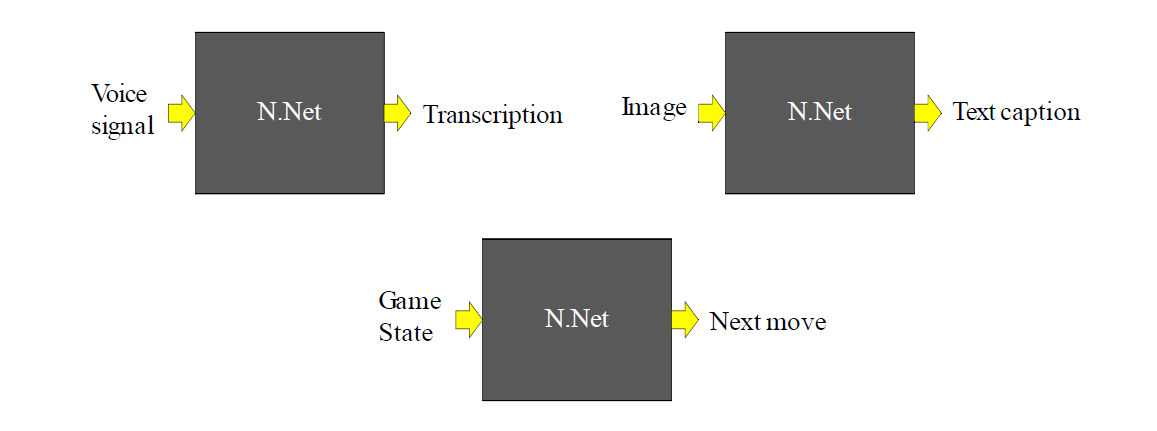
\includegraphics[width=0.9\linewidth]{images/nn_as_function.png}
        \caption{Neural networks act as functions mapping inputs (like voice or images) to outputs (like text or actions).}
    \end{figure}
\end{frame}

\begin{frame}{The Goal: The Formal Problem Setup}
    \framesubtitle{What we have and what we want}
    Based on the previous slides, we can formally define our task:
    \begin{itemize}
        \item \textbf{Given:}
        \begin{itemize}
            \item The \bhighlight{architecture} of the network (e.g., number of layers and neurons).
            \item A set of N \bhighlight{training data} pairs: $(x^{(1)}, y^{(1)}), (x^{(2)}, y^{(2)}), \dots, (x^{(N)}, y^{(N)})$.
        \end{itemize}
        \medskip
        \item \textbf{To Find:}
        \begin{itemize}
            \item The optimal set of \bhighlight{parameters} (weights and biases, denoted collectively as $W$) for our network.
        \end{itemize}
    \end{itemize}
\end{frame}

% --- SLIDE WITH CORRECTION ---
\begin{frame}{The Goal: The Parametric Function and Cost} 
    \framesubtitle{Representing the Network and its Error}
    \begin{itemize}
        \item We consider a neural network as a \bhighlight{parametric function}, $f(x; W)$, where $W$ represents all learnable parameters.
        \item A \bhighlight{loss function}, $\text{loss}(f(x;W), y)$, penalizes the difference between the network's prediction and the desired output for a \emph{single} training example.
        \item The overall \bhighlight{Cost Function} $E(W)$ is the average loss over the \emph{entire} dataset:
        \[
            E(W) = \frac{1}{N} \sum_{n=1}^{N} \text{loss}(f(x^{(n)}; W), y^{(n)})
        \]
    \end{itemize}
\end{frame}

\begin{frame}{The Goal: A Key Requirement}
    \framesubtitle{The Need for Differentiability}
    \begin{itemize}
        \item Our goal is to minimize the cost $E(W)$. To do this with gradient-based methods, the cost function must be \bhighlight{differentiable} with respect to the weights $W$.
        \item This means we must use:
        \begin{itemize}
            \item \textbf{Differentiable Loss Functions:} The way we measure error must be smooth.
            \item \textbf{Continuous Activation Functions:} The functions inside our neurons (like Sigmoid or ReLU) must be differentiable, allowing gradients to flow through the network.
        \end{itemize}
    \end{itemize}
\end{frame}

\begin{frame}{Case Study: Regression}
    \framesubtitle{Output and Loss for Real-Valued Targets}
    \begin{itemize}
        \item For tasks where the desired output is a real number or a vector of real numbers (e.g., predicting a price).
        \item \textbf{Output Layer:} Typically has linear neurons (i.e., no activation function is applied).
        \item \textbf{Loss Function:} The most common choice is the \bhighlight{Squared Error} (or L2 loss):
        \[
            \text{loss}(y, o) = \frac{1}{2} \|y - o\|^2 = \frac{1}{2} \sum_k (y_k - o_k)^2
        \]
    \end{itemize}
    \begin{figure}
        \centering
        % Source: MLP & Back-prop.pdf, Page: 7
        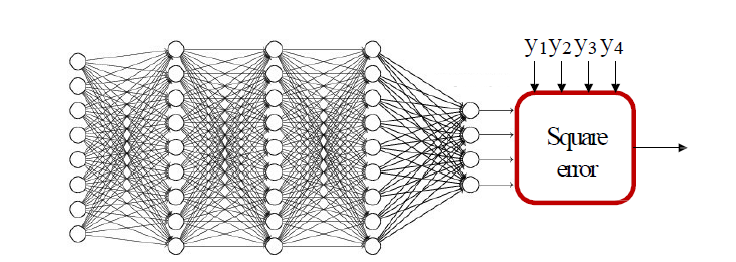
\includegraphics[width=0.8\linewidth]{images/loss_regression.png}
    \end{figure}
\end{frame}

\begin{frame}{Case Study: Binary Classification}
    \framesubtitle{Output and Loss for Two-Class Problems}
    \begin{itemize}
        \item For tasks with two classes (e.g., Cat vs. Dog), where the target $y$ is either 0 or 1.
        \item \textbf{Output Layer:} A single neuron with a \bhighlight{Sigmoid} activation function. This squashes the output to a range of (0, 1), which we can interpret as a probability $P(Y=1|x)$.
        \item \textbf{Loss Function:} \bhighlight{Binary Cross-Entropy} is the standard choice:
        \[
            \text{loss}(y, o) = -y \log(o) - (1 - y) \log(1 - o)
        \]
    \end{itemize}
    \begin{figure}
        \centering
        % Source: MLP & Back-prop.pdf, Page: 11
        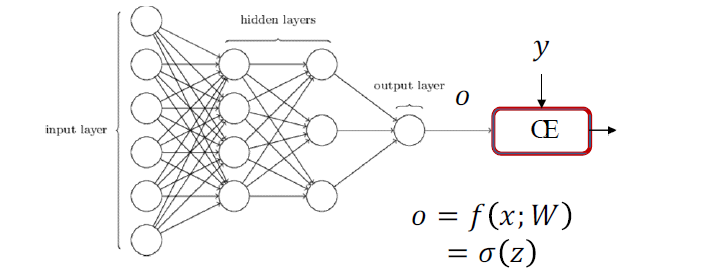
\includegraphics[width=0.6\linewidth]{images/loss_binary_ce.png}
    \end{figure}
\end{frame}

\begin{frame}{Case Study: Multi-Class Classification}
    \framesubtitle{Setup for K > 2 Classes}
    \begin{itemize}
        \item For tasks with multiple classes (e.g., MNIST digits 0-9).
        \item \textbf{Target Representation:} The desired output $y$ is represented as a \bhighlight{one-hot vector}. For example, for class 3 out of 5, $y = [0, 0, 1, 0, 0]^T$.
        \item \textbf{Output Layer:} Must have K neurons, one for each class.
        \item To ensure the outputs are probabilities that sum to 1, we need a special activation function.
    \end{itemize}
\end{frame}

\begin{frame}{Case Study: Multi-Class Classification}
    \framesubtitle{The Softmax Activation}
    \begin{itemize}
        \item The \bhighlight{Softmax} function is used as the activation for the output layer in multi-class problems.
        \item It takes a vector of raw scores (logits) $z$ and transforms it into a probability distribution $o$:
        \[
            o_i = \text{softmax}(z)_i = \frac{\exp(z_i)}{\sum_{j=1}^{K} \exp(z_j)}
        \]
        \item Each output $o_i$ is between 0 and 1, and all outputs sum to 1, making them valid probabilities.
    \end{itemize}
    \begin{figure}
        \centering
        % Source: MLP & Back-prop.pdf, Page: 13
        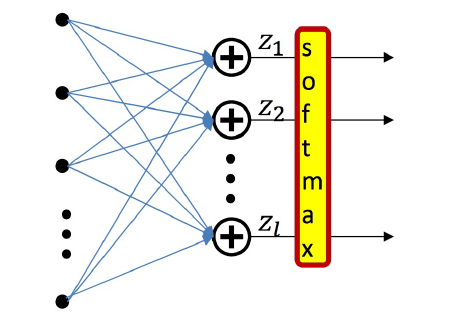
\includegraphics[width=0.5\linewidth]{images/softmax_layer.png}
        \caption{The softmax activation is applied to the final layer.}
    \end{figure}
\end{frame}

\begin{frame}{Case Study: Multi-Class Classification}
    \framesubtitle{Cross-Entropy Loss}
    \begin{itemize}
        \item \textbf{Loss Function:} For multi-class classification, we use the \bhighlight{Cross-Entropy} loss.
        \[
            \text{loss}(y, o) = -\sum_{i=1}^{K} y_i \log(o_i)
        \]
        \item Since $y$ is a one-hot vector, only one term in the sum is non-zero. If the true class is $c$, the formula simplifies to:
        \[
            \text{loss}(y, o) = - \log(o_c)
        \]
        \item This means we are trying to maximize the log-probability of the correct class.
    \end{itemize}
    \begin{figure}
        \centering
        % Source: MLP & Back-prop.pdf, Page: 15
        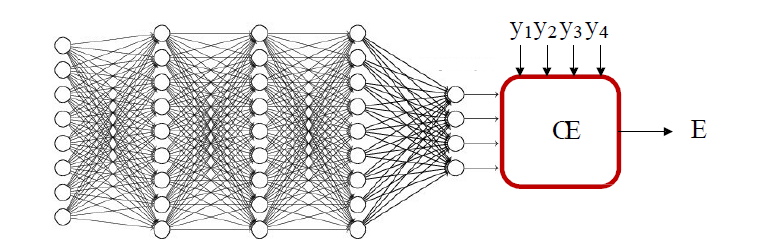
\includegraphics[width=0.8\linewidth]{images/loss_multiclass_ce.png}
    \end{figure}
\end{frame}
\begin{frame}{The Tool: Gradient Descent}
    \framesubtitle{The Core Idea}
    \begin{itemize}
        \item We use an iterative optimization algorithm called \bhighlight{gradient descent} to find the minimum of the cost function.
        \item The core idea is to take steps in the direction of the \bhighlight{negative gradient} of the error surface, effectively moving "downhill" to find a minimum.
    \end{itemize}
    \begin{figure}
        \centering
        % Source: Optimization II.pdf, Page: 2
        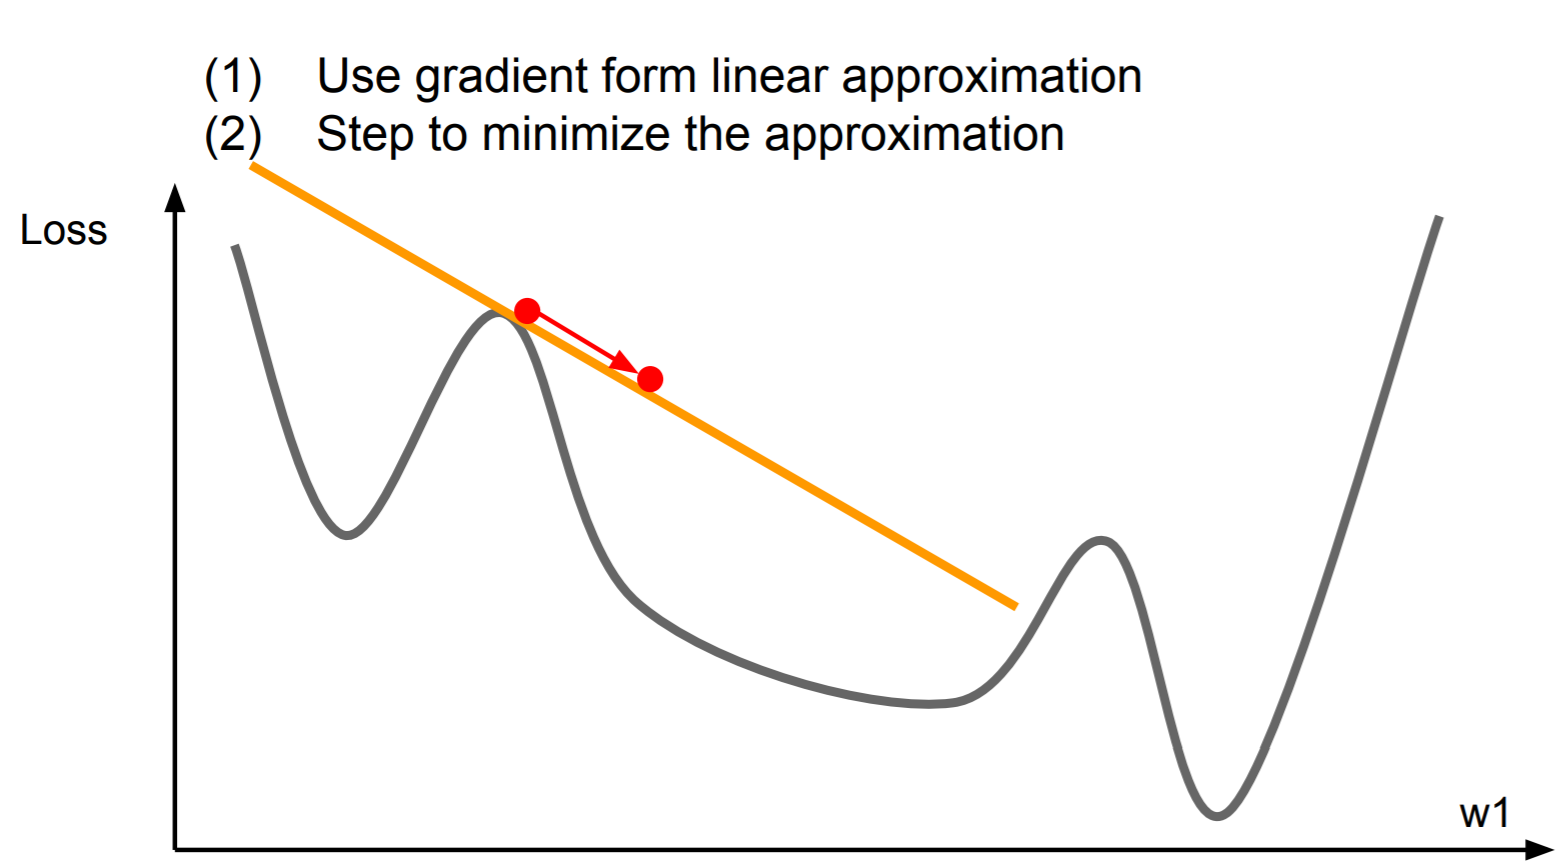
\includegraphics[width=0.7\linewidth]{images/gradient_descent_step.png} 
        \caption{A single step of gradient descent. We form a linear approximation of the loss and step to minimize it.}
    \end{figure}
\end{frame}

\begin{frame}{The Tool: Gradient Descent}
    \framesubtitle{The Update Rule}
    \begin{itemize}
        \item At each step, we update the weights according to the following rule:
        \[
            w^{t+1} = w^{t} - \eta \nabla_{w}J(w^{t})
        \]
        \item Where:
        \begin{itemize}
            \item $w^{t}$ is the vector of weights at step $t$.
            \item $\eta$ (eta) is the \bhighlight{learning rate}, a hyperparameter that controls the step size.
            \item $\nabla_{w}J(w^{t})$ is the gradient of the cost function with respect to the weights.
        \end{itemize}
    \end{itemize}
\end{frame}

\begin{frame}{The Tool: Gradient Descent}
    \framesubtitle{Calculating the Gradient}
    \begin{itemize}
        \item The gradient $\nabla_{w}J$ is computed efficiently using the \bhighlight{backpropagation} algorithm.
        \item Backpropagation is essentially a recursive application of the \bhighlight{chain rule} from calculus to compute the gradient for every parameter in the network.
        \item The process involves two main steps:
        \begin{enumerate}
            \item A \bhighlight{forward pass} to compute the network's output and the final loss.
            \item A \bhighlight{backward pass} to propagate the error gradients from the output layer back to the input layer, calculating the gradient for each weight along the way.
        \end{enumerate}
    \end{itemize}
\end{frame}
\begin{frame}{The Computational Graph}
    \framesubtitle{Why do we need them?}
    \begin{itemize}
        \item As we've seen, the output of a neural network is a deeply nested composite function.
        \item To calculate the gradient of the loss with respect to any weight, we must use the \bhighlight{chain rule} from calculus.
        \item For a network with millions of parameters, applying the chain rule manually is impossible. A \bhighlight{computational graph} is a powerful visualization tool that helps us manage this complexity and automate the process.
    \end{itemize}
\end{frame}

\begin{frame}{The Computational Graph}
    \framesubtitle{Structure}
    \begin{itemize}
        \item A computational graph represents a function as a directed graph:
        \begin{itemize}
            \item \bhighlight{Nodes (Vertices):} Represent operations (e.g., addition, multiplication) or variables.
            \item \bhighlight{Edges:} Represent the flow of data. The output of one node becomes the input to another.
        \end{itemize}
    \end{itemize}
    \begin{figure}
        \centering
        % Source: MLP & Back-prop.pdf, Page: 40
        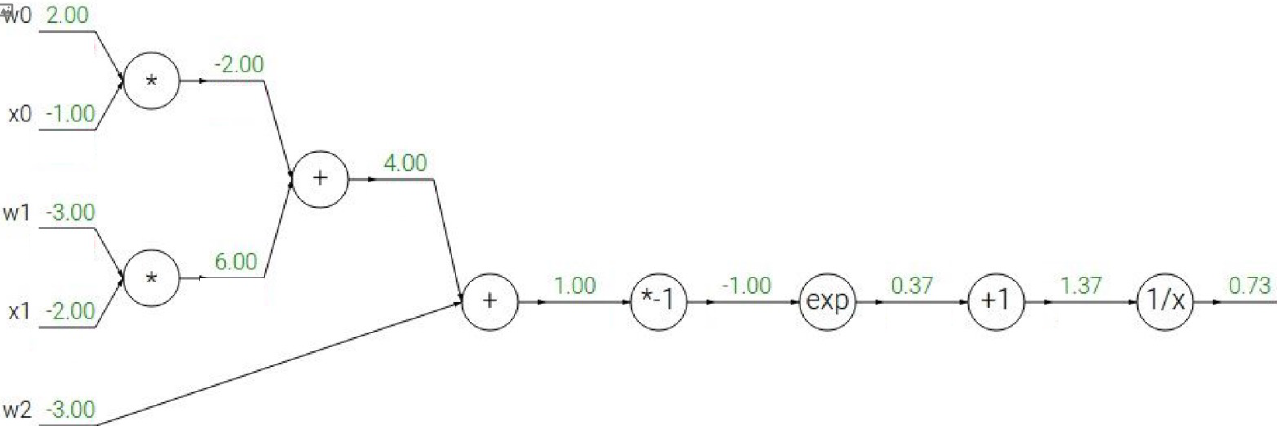
\includegraphics[width=0.9\linewidth]{images/computational_graph_sigmoid_forward.png}
        \caption{A computational graph breaking down a sigmoid neuron into its elementary operations.}
    \end{figure}
\end{frame}

\begin{frame}{The Computational Graph}
    \framesubtitle{The Forward Pass}
    \begin{itemize}
        \item The \bhighlight{forward pass} is the process of evaluating the function represented by the graph.
        \item We start from the input nodes and move forward through the graph, applying the operation at each node to the incoming values.
        \item This continues until we reach the final node, which typically represents the overall loss of the network. The path is determined by the topological sort of the graph's nodes.
    \end{itemize}
    \begin{center}
        \begin{minipage}{0.8\textwidth}
        \begin{figure}
            \centering
            % Source: MLP & Back-prop.pdf, Page: 40
            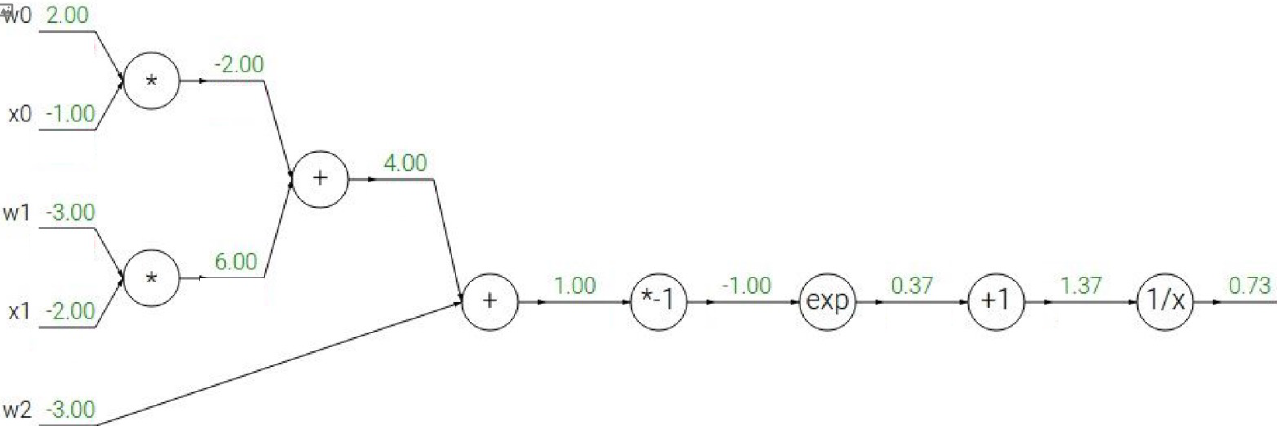
\includegraphics[width=\linewidth]{images/computational_graph_sigmoid_forward.png}
            \caption{In the forward pass, values are computed from left to right. For example, $w_0 \times x_0 = 2.00 \times -1.00 = -2.00$.}
        \end{figure}
        \end{minipage}
    \end{center}
\end{frame}

\begin{frame}{The Computational Graph}
    \framesubtitle{The Backward Pass and The Chain Rule}
    \begin{itemize}
        \item \bhighlight{Backpropagation} is the process of calculating the gradients by moving backward through the graph.
        \item At each node, we use the chain rule to compute the gradient of the final loss with respect to the node's \emph{inputs}, given the gradient with respect to its \emph{output}.
        \item We define three key terms:
        \begin{itemize}
            \item \bhighlight{Upstream Gradient ($\frac{\partial L}{\partial z}$):} The gradient coming from the nodes that follow.
            \item \bhighlight{Local Gradient ($\frac{\partial z}{\partial x}$):} The derivative of the node's operation with respect to its own inputs.
            \item \bhighlight{Downstream Gradient ($\frac{\partial L}{\partial x}$):} The gradient we want to compute and pass backward.
        \end{itemize}
        \[
            \text{Downstream Gradient} = \text{Upstream Gradient} \times \text{Local Gradient}
        \]
    \end{itemize}
\end{frame}

\begin{frame}{The Computational Graph}
    \framesubtitle{Example "Gates"}
    \begin{itemize}
        \item Different nodes (or "gates") distribute the upstream gradient in unique ways based on their local gradient:
    \end{itemize}
    \begin{figure}
        \centering
        % Source: MLP & Back-prop.pdf, Page: 38
        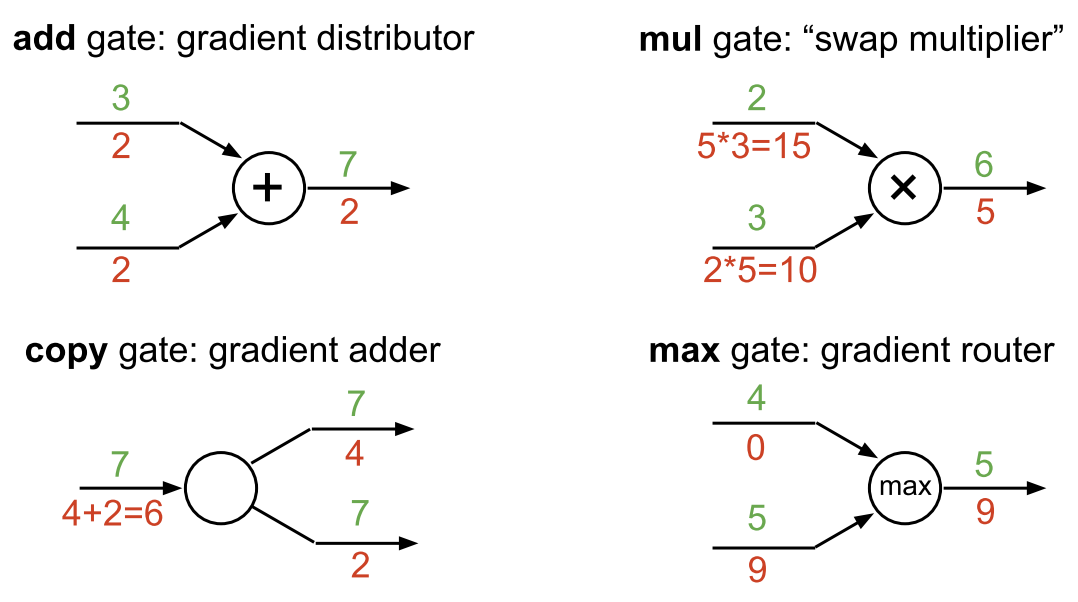
\includegraphics[width=\linewidth]{images/gradient_gates.png}
        \caption{
            \textbf{Add gate:} acts as a "gradient distributor".
            \textbf{Max gate:} acts as a "gradient router".
            \textbf{Multiply gate:} acts as a "swap multiplier".
        }
    \end{figure}
\end{frame}

\begin{frame}{The Computational Graph}
    \framesubtitle{Backpropagation Example: Step 1}
    \begin{itemize}
        \item Let's trace the backward pass for our sigmoid neuron example.
        \item We start at the very end. The gradient of the output with respect to itself is \bhighlight{1}. This is our initial upstream gradient.
    \end{itemize}
    \begin{figure}
        \centering
        % Source: MLP & Back-prop.pdf, Pages: 41-42 (combined view)
        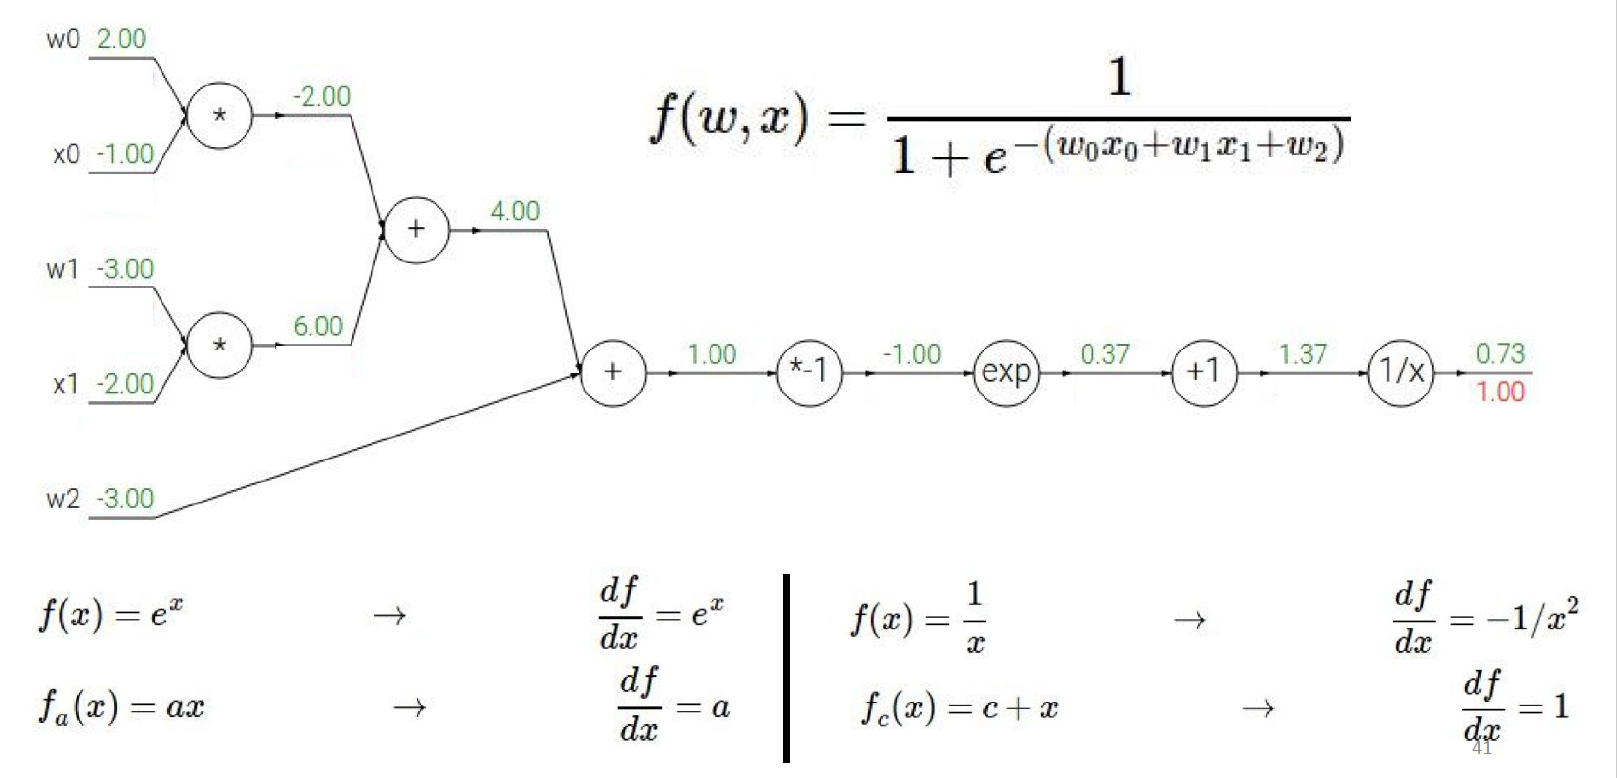
\includegraphics[width=\linewidth]{images/sigmoid_backprop_1.png}
        \caption{Starting the backward pass. The initial gradient at the output is 1.}
    \end{figure}
\end{frame}

\begin{frame}{The Computational Graph}
    \framesubtitle{Backpropagation Example: Step 2}
    \begin{itemize}
        \item The first gate is the $1/x$ gate.
        \item \textbf{Upstream Gradient}: 1.0
        \item \textbf{Local Gradient}: The derivative of $f(x) = 1/x$ is $-1/x^2$. Since the input was 1.37, the local gradient is $-1/(1.37^2) \approx -0.53$.
        \item \textbf{Downstream Gradient}: $1.0 \times -0.53 = -0.53$.
    \end{itemize}
    \begin{figure}
        \centering
        % Source: MLP & Back-prop.pdf, Page: 43
        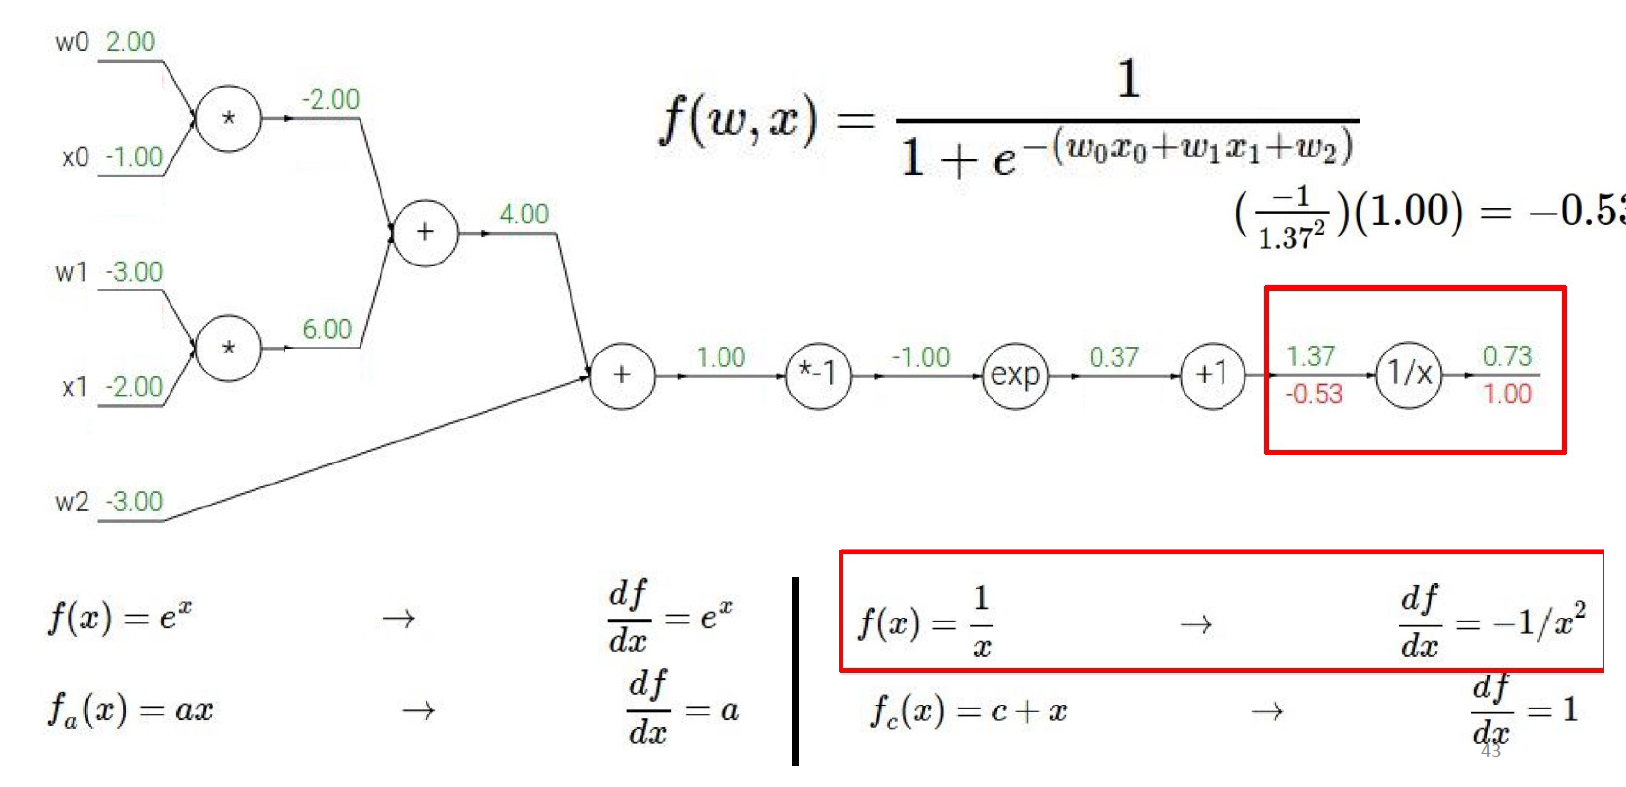
\includegraphics[width=\linewidth]{images/sigmoid_backprop_2.png}
    \end{figure}
\end{frame}

\begin{frame}{The Computational Graph}
    \framesubtitle{Backpropagation Example: Step 3}
    \begin{itemize}
        \item The next gate is the `+1` gate.
        \item \textbf{Upstream Gradient}: -0.53
        \item \textbf{Local Gradient}: The derivative of $f(x) = x+c$ is 1.
        \item \textbf{Downstream Gradient}: $-0.53 \times 1 = -0.53$.
    \end{itemize}
    \begin{figure}
        \centering
        % Source: MLP & Back-prop.pdf, Page: 45
        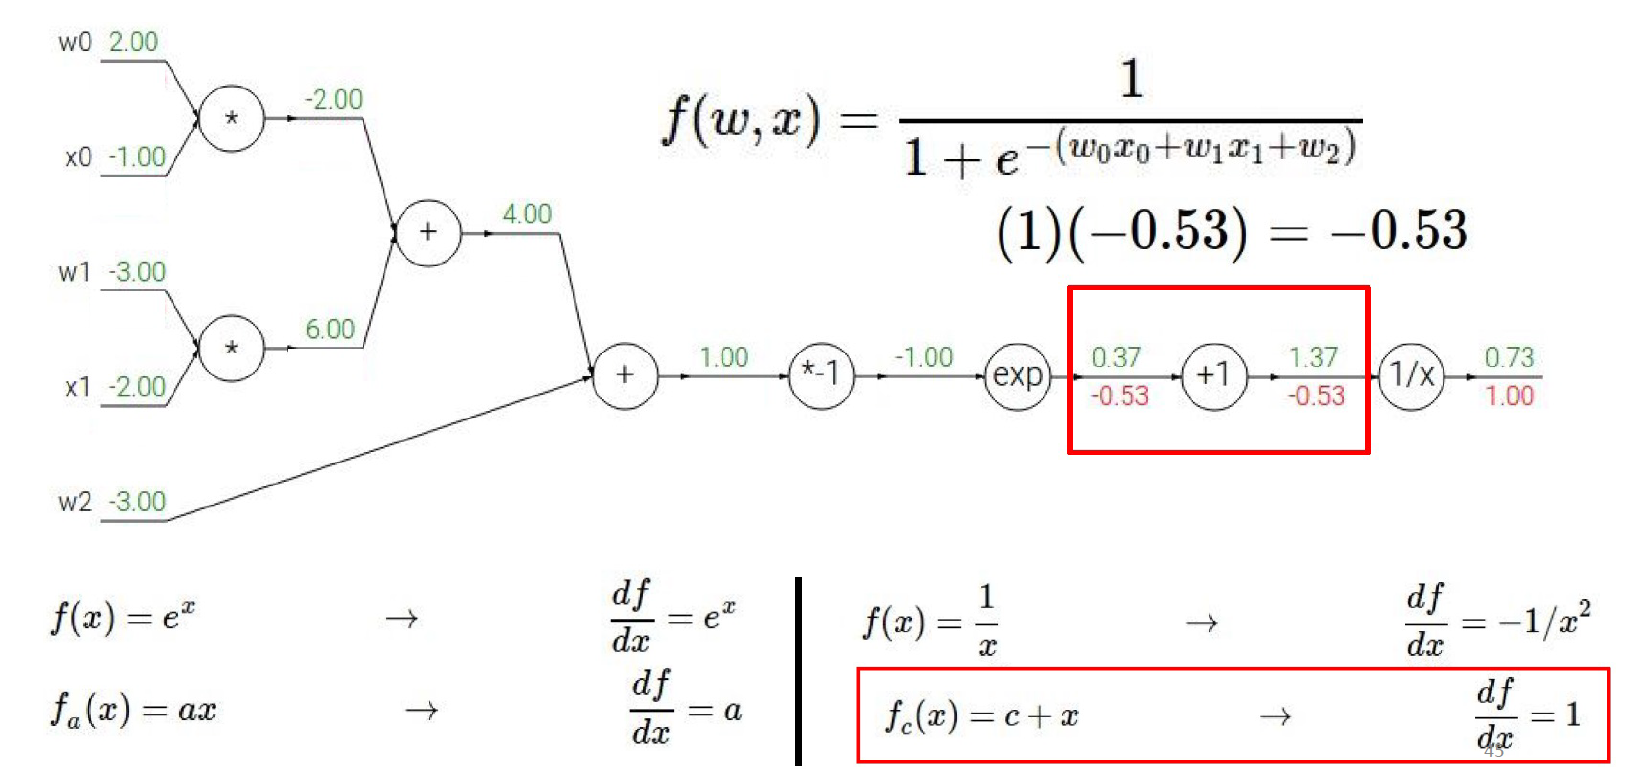
\includegraphics[width=\linewidth]{images/sigmoid_backprop_3.png}
    \end{figure}
\end{frame}

\begin{frame}{The Computational Graph}
    \framesubtitle{Backpropagation Example: Step 4}
    \begin{itemize}
        \item Next is the `exp` gate.
        \item \textbf{Upstream Gradient}: -0.53
        \item \textbf{Local Gradient}: The derivative of $f(x) = e^x$ is $e^x$. Since the input was -1.0, the local gradient is $e^{-1} \approx 0.37$.
        \item \textbf{Downstream Gradient}: $-0.53 \times 0.37 \approx -0.20$.
    \end{itemize}
    \begin{figure}
        \centering
        % Source: MLP & Back-prop.pdf, Page: 48
        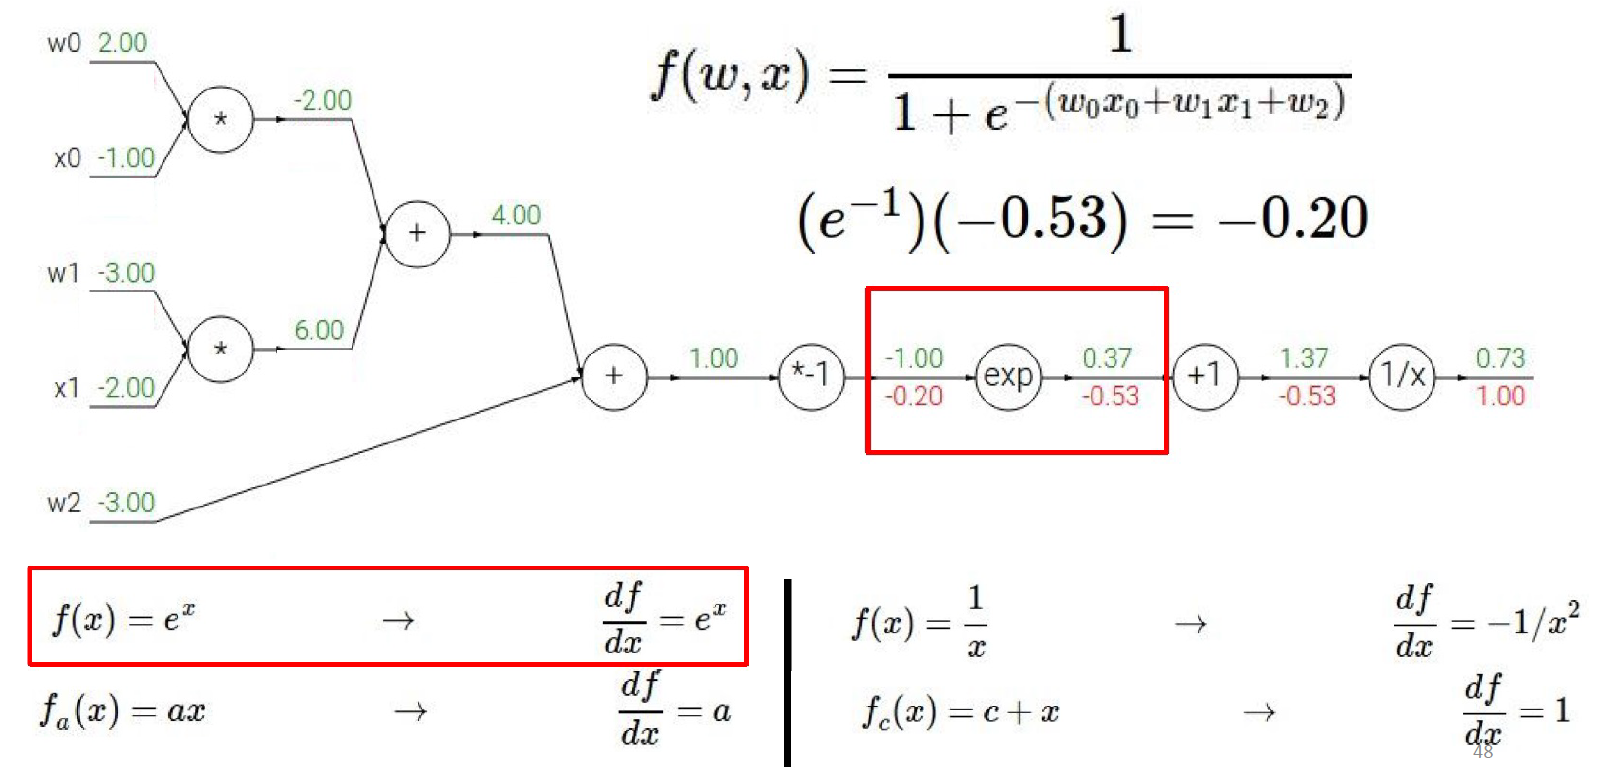
\includegraphics[width=\linewidth]{images/sigmoid_backprop_4.png}
    \end{figure}
\end{frame}

\begin{frame}{The Computational Graph}
    \framesubtitle{Backpropagation Example: Final Steps}
    \begin{itemize}
        \item The gradient is propagated backward through the remaining gates (`*-1`, `+`, `*`).
        \item For example, at the top-most `*` gate (for $w_0, x_0$):
        \begin{itemize}
            \item \textbf{Upstream Gradient}: 0.20 (from the final `+` gate).
            \item \textbf{Local Gradient} for $w_0$: The other input, $x_0 = -1.00$.
            \item \textbf{Downstream Gradient} for $w_0$: $0.20 \times -1.00 = -0.20$.
        \end{itemize}
        \item This process is repeated until we have the gradient for every weight and input.
    \end{itemize}
    \begin{figure}
        \centering
        % Source: MLP & Back-prop.pdf, Page: 53
        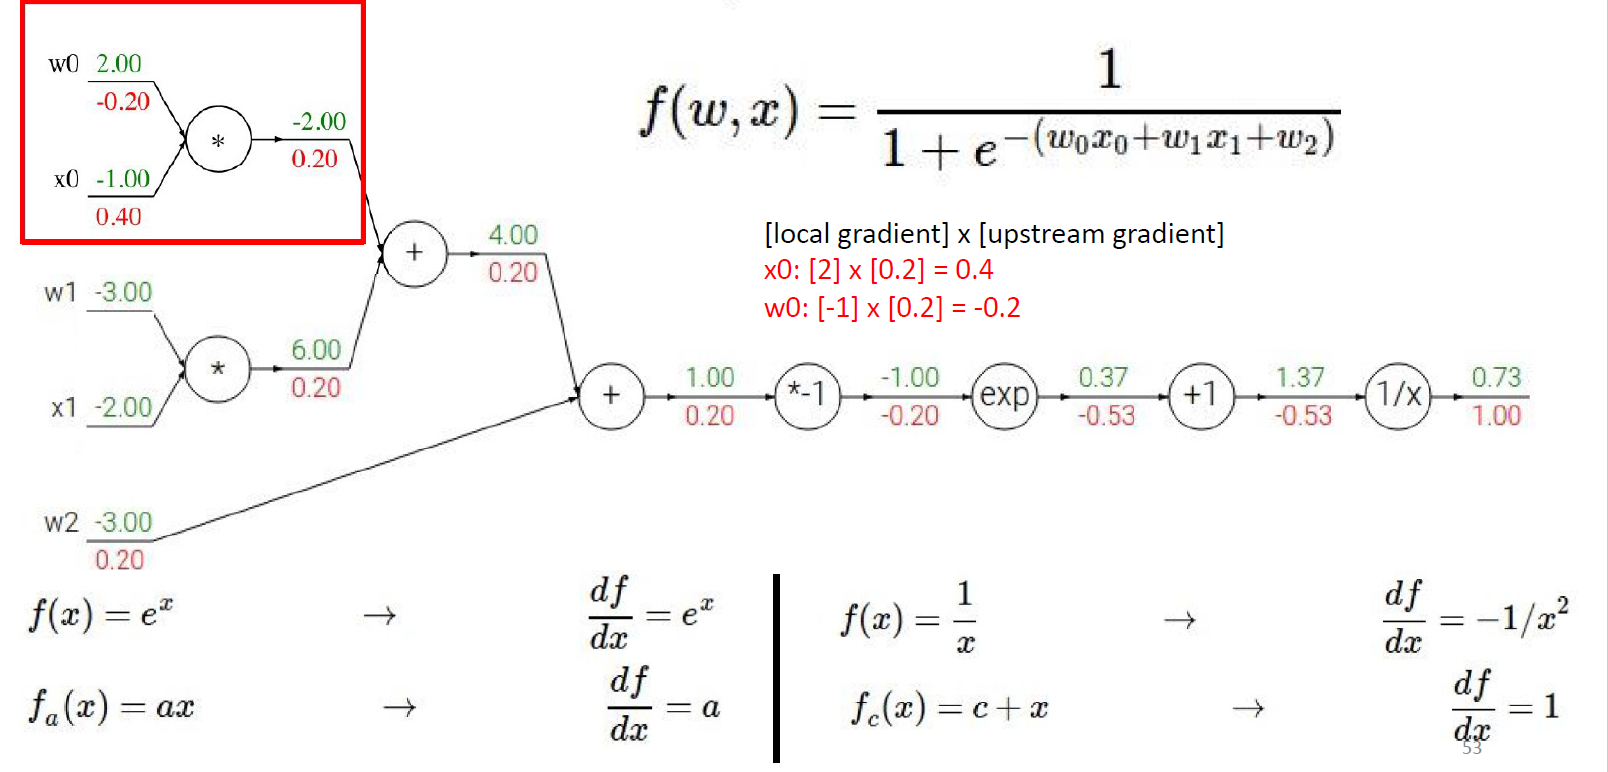
\includegraphics[width=\linewidth]{images/sigmoid_backprop_final.png}
        \caption{The final computed gradients for each weight and input.}
    \end{figure}
\end{frame}
\begin{frame}{From Scalars to Vectors}
    \framesubtitle{Efficient Implementation}
    \begin{itemize}
        \item While the computational graph concept works for single values (scalars), neural networks are implemented using \bhighlight{vectors and matrices} for efficiency.
        \item Instead of calculating gradients one by one, we can process an entire layer or even a mini-batch of data with a few matrix operations.
    \end{itemize}
\end{frame}

\begin{frame}{From Scalars to Vectors}
    \framesubtitle{The Jacobian Matrix}
    \begin{columns}[c]
        \begin{column}{0.5\linewidth}
            \begin{itemize}
                \item The derivative of a vector function with respect to a vector input is a matrix of all possible partial derivatives, called the \bhighlight{Jacobian}.
                \item For a layer's activation $a = f(z)$, the Jacobian $\frac{\partial a}{\partial z}$ tells us how a small change in each input element $z_i$ affects each output element $a_j$.
            \end{itemize}
        \end{column}
        \begin{column}{0.5\linewidth}
            \begin{figure}
                \centering
                % Source: MLP & Back-prop.pdf, Page: 73
                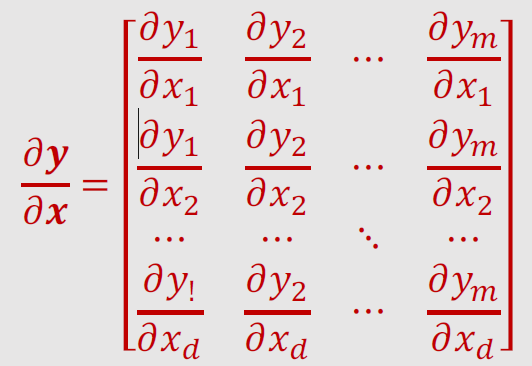
\includegraphics[width=0.8\linewidth]{images/jacobian_matrix.png}
                \caption{Structure of a Jacobian matrix.}
            \end{figure}
        \end{column}
    \end{columns}
\end{frame}

\begin{frame}{From Scalars to Vectors}
    \framesubtitle{Vectorized Forward \& Backward Pass}
    \begin{itemize}
        \item \textbf{Forward Pass:} For a layer $l$, we compute the pre-activation $z^{[l]}$ and activation $a^{[l]}$ for all neurons at once:
        \[ z^{[l]} = W^{[l]}a^{[l-1]} \quad , \quad a^{[l]} = f(z^{[l]}) \]
        \item \textbf{Backward Pass:} We propagate a "sensitivity" or error vector $\delta^{[l]} = \frac{\partial \text{Loss}}{\partial z^{[l]}}$. This vector is passed backward using the chain rule:
        \[ \delta^{[l-1]} = (W^{[l]T}\delta^{[l]}) \odot f'(z^{[l-1]}) \]
        where $\odot$ is element-wise multiplication.
    \end{itemize}
\end{frame}

\begin{frame}{From Scalars to Vectors}
    \framesubtitle{Vectorized Gradient Calculation}
    \begin{itemize}
        \item Once we have the sensitivity vector $\delta^{[l]}$, the gradient for the entire weight matrix of that layer can be computed with a single matrix operation:
        \[ \frac{\partial \text{Loss}}{\partial W^{[l]}} = \delta^{[l]}(a^{[l-1]})^{T} \]
        \item This vectorized approach is significantly more efficient than looping through individual weights.
    \end{itemize}
    \begin{figure}
        \centering
        % Source: MLP & Back-prop.pdf, Page: 63
        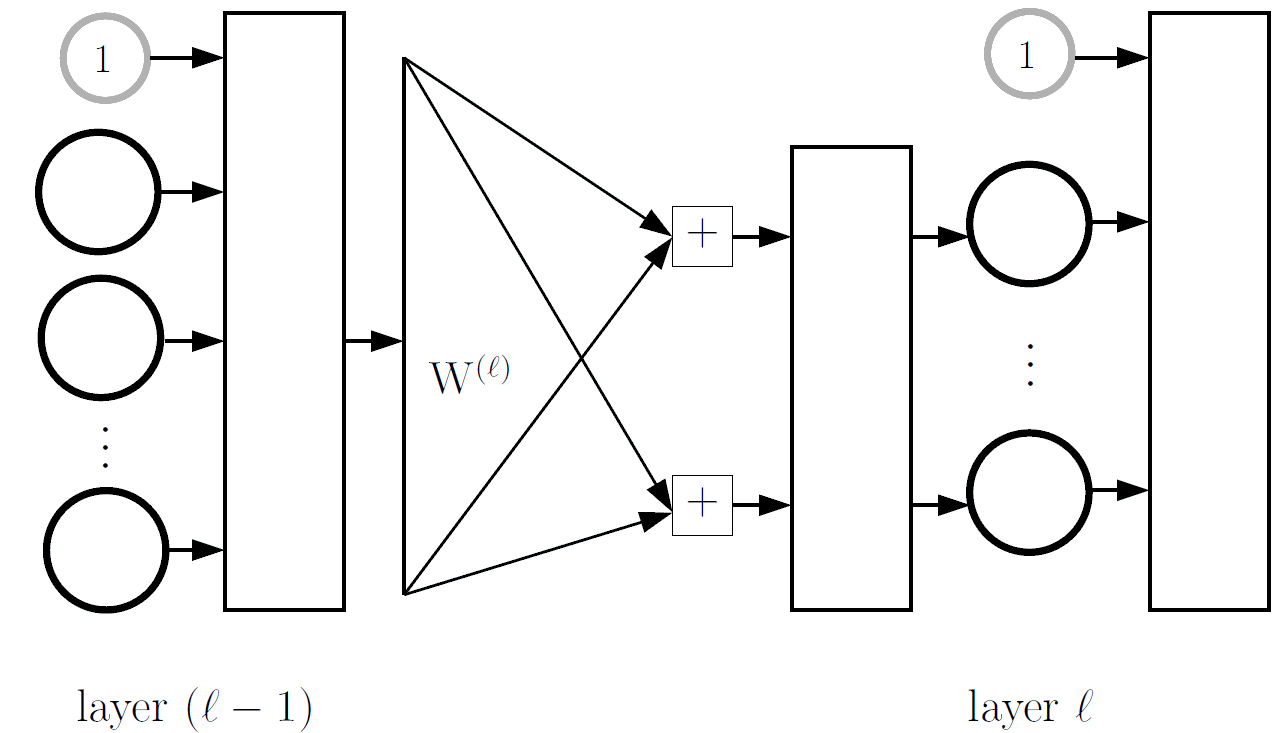
\includegraphics[width=0.8\linewidth]{images/vectorized_backprop.png}
        \caption{Vectorized data flow from the activations of the previous layer ($a^{[l-1]}$) to the current layer ($a^{[l]}$).}
    \end{figure}
\end{frame}

\begin{frame}{The Landscape: Challenges of the Error Surface}
    \begin{itemize}
        \item The error surface for deep networks is complex and \bhighlight{non-convex}, presenting several challenges for gradient descent.
        \item \textbf{Local Minima:} These are points where the gradient is zero, but which are not the global minimum. While a concern, they are less of a problem in high-dimensional spaces than saddle points.
        \item \textbf{Saddle Points:} These are points where the gradient is also zero, but the function curves up in some directions and down in others. Gradient descent can get "stuck" and slow down significantly on them.
    \end{itemize}
    \begin{figure}
        \centering
        % Source: Optimization I.pdf, Page: 3
        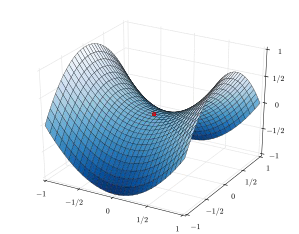
\includegraphics[width=0.4\linewidth]{images/saddle_point.png}
        \caption{A visualization of a saddle point.}
    \end{figure}
\end{frame}

\begin{frame}{The Landscape: Challenges of the Error Surface}
    \framesubtitle{Saddle Points vs. Local Minima}
    \begin{itemize}
        \item A popular and important hypothesis in deep learning is that in large networks, \bhighlight{saddle points are far more common} than local minima.
        \item For a point to be a local minimum, the curvature must be positive in \emph{all} dimensions. For a high-dimensional space, the probability of this is very low.
        \item Therefore, most points with zero gradient that our optimizer finds are likely to be saddle points, not "bad" local minima.
    \end{itemize}
    \begin{figure}
        \centering
        % Source: Optimization I.pdf, Page: 4
        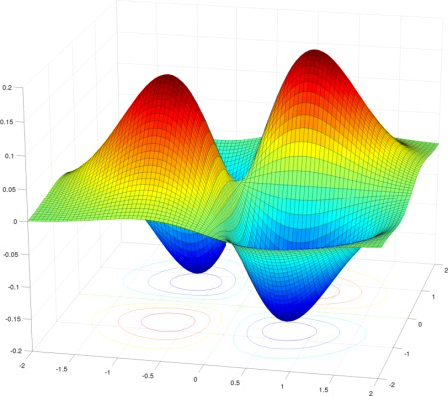
\includegraphics[width=0.5\linewidth]{images/error_surfaces.png}
        \caption{Examples of complex, non-convex error surfaces in neural networks.}
    \end{figure}
\end{frame}
\section{Advanced Optimization}

\subsection{The Problem of Poor Conditioning}

\begin{frame}{The Problem of Poor Conditioning}
    \framesubtitle{The Challenge of the Error Surface}
    \begin{itemize}
        \item The error surface of a neural network can have very different curvature along different directions.
        \item When the contours of the error surface are elongated ellipsoids, the problem is said to be \textbf{poorly conditioned} or \textbf{ill-conditioned}.
        \item This creates a scenario resembling a long, narrow valley.
    \end{itemize}
    \begin{figure}
        % Placeholder for the elongated ellipsoid visualization from Optimization I.pdf, p. 18
        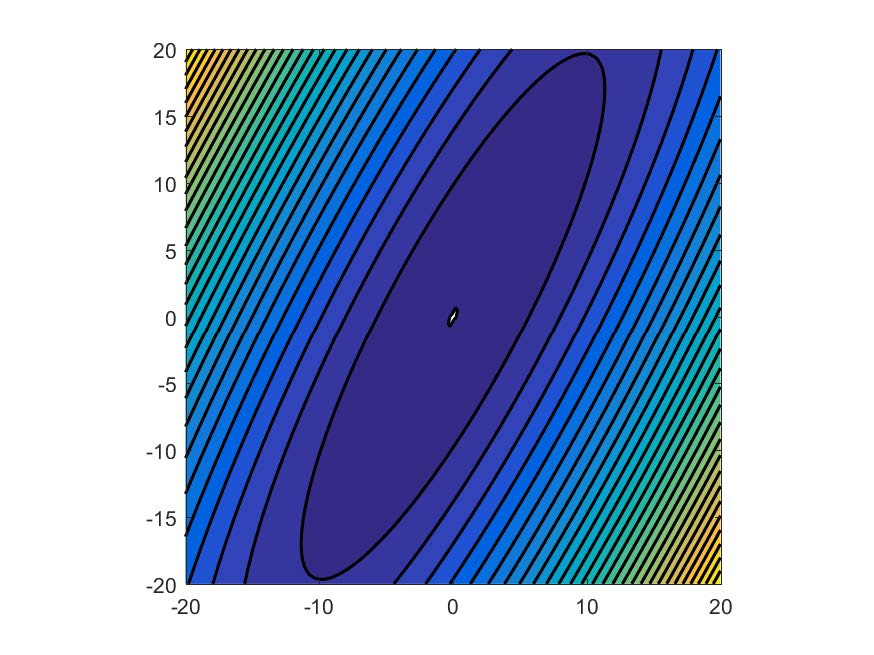
\includegraphics[width=0.5\textwidth]{images/elongated_ellipsoid.jpeg}
        \caption{An ill-conditioned error surface with elliptical contour lines.}
    \end{figure}
\end{frame}

\begin{frame}{Consequences of Poor Conditioning}
    \framesubtitle{Inefficient Gradient Descent}
    A single learning rate struggles on an ill-conditioned surface.
    \begin{itemize}
        \item The gradient vector is always perpendicular to the contour lines.
        \item In a narrow valley, this means the gradient points mostly across the valley, not along it.
        \item \textbf{Result:} The optimization path "zig-zags" inefficiently.
        \begin{itemize}
            \item \textbf{Fast oscillations} across the steep direction (the valley walls).
            \item \textbf{Slow progress} along the shallow direction (the valley floor).
        \end{itemize}
    \end{itemize}
    \begin{figure}
        % Placeholder for the oscillating gradient descent path from Optimization I.pdf, p. 18
        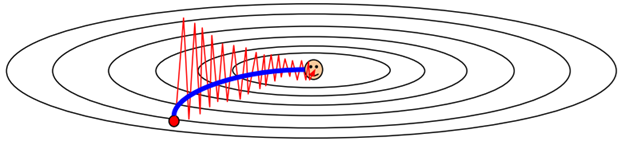
\includegraphics[width=1\textwidth]{images/zigzag.png}
        \caption{Gradient descent oscillates in the steep direction while making slow progress in the shallow direction.}
    \end{figure}
\end{frame}

\begin{frame}{The Learning Rate Dilemma}
    \framesubtitle{One Step Size, Two Different Needs}
    The core issue is that different directions require different optimal learning rates.
    \begin{itemize}
        \item To prevent divergence, the learning rate $\eta$ must be small enough for the steepest direction.
        \item This small learning rate is then far too small for the shallow direction, leading to extremely slow convergence.
        \item This conflict forces a compromise that is suboptimal for all directions.
    \end{itemize}
    \begin{alertblock}{The Motivation for Advanced Optimizers}
        Poor conditioning is a key reason that vanilla gradient descent is often too slow. This motivates methods that can adapt and take appropriately sized steps in different directions.
    \end{alertblock}
\end{frame}

\subsection{Second-Order Optimization (Newton's Method)}

\begin{frame}{The Limits of First-Order Methods}
    \framesubtitle{The Problem with a Single Learning Rate}
    \begin{itemize}
        \item Vanilla Gradient Descent uses a single learning rate for all parameters.
        \item On ill-conditioned error surfaces (long, narrow valleys), this is inefficient.
        \item The learning rate is either too large for steep directions (causing oscillation) or too small for shallow directions (causing slow progress).
        \item \textbf{Question:} Can we do better by using information about the surface's curvature?
    \end{itemize}
\end{frame}

\begin{frame}{Second-Order Optimization: The Idea}
    \framesubtitle{Using Curvature for Faster Convergence}
    Instead of a linear approximation, second-order methods use a local \textbf{quadratic approximation} of the loss function.
    \begin{itemize}
        \item This is based on the second-order Taylor expansion for loss function E($w$) around the current point $w^{(k)}$:
        \begin{equation*}
        \begin{split}
            E(w) \approx E(w^{(k)}) &+ \nabla_{w}E(w^{(k)})^{T}(w-w^{(k)}) \\
            &+ \frac{1}{2}(w-w^{(k)})^{T}H_{E}(w^{(k)})(w-w^{(k)})
        \end{split}
        \end{equation*}
        \item \textbf{Newton's Method} jumps directly to the minimum of this quadratic approximation in a single step.
    \end{itemize}
    \begin{figure}
        % Placeholder for the Newton's method visualization from Optimization II.pdf, p. 4
        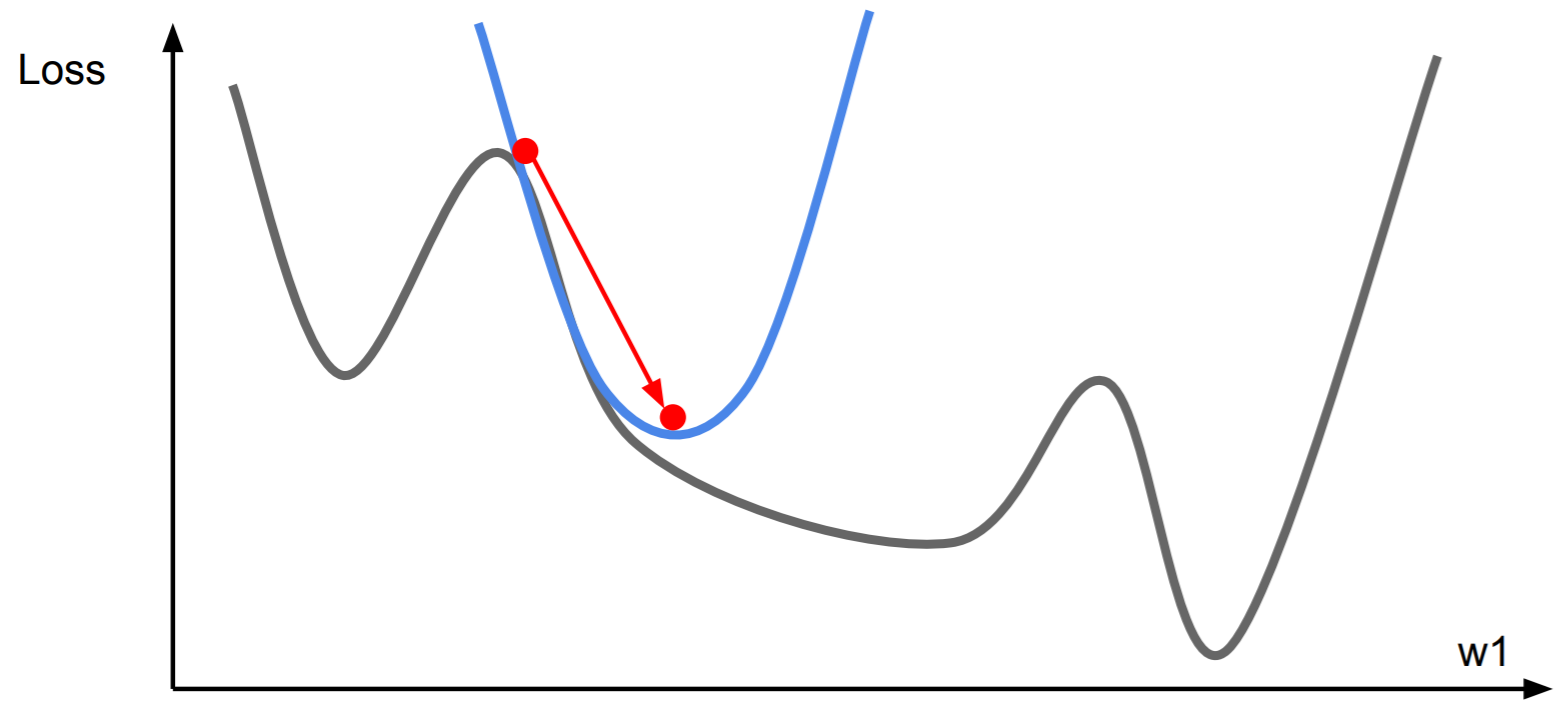
\includegraphics[width=0.5\textwidth]{images/secondmethods.png}
        \caption{Newton's method forms a local quadratic approximation (blue) and jumps to its minimum.}
    \end{figure}
\end{frame}

\begin{frame}{Second-Order Optimization: The Idea}
    \framesubtitle{Intuition Behind Newton's Method}
    \begin{figure}
        \centering
        \begin{minipage}{.5\textwidth}
            \centering
            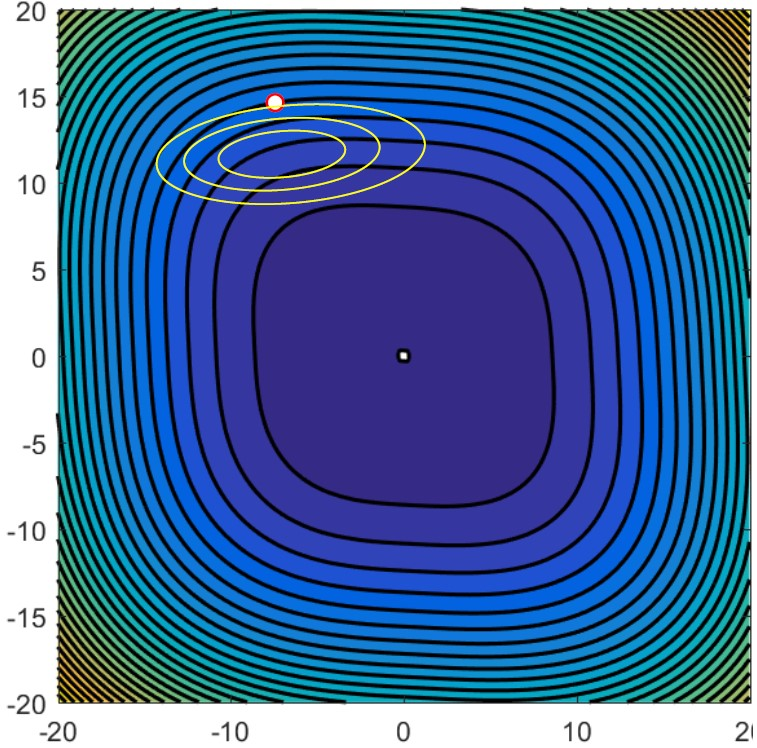
\includegraphics[width=\textwidth]{images/intuition_newton1.jpeg}
        \end{minipage}%
            \begin{minipage}{.5\textwidth}
            \centering
            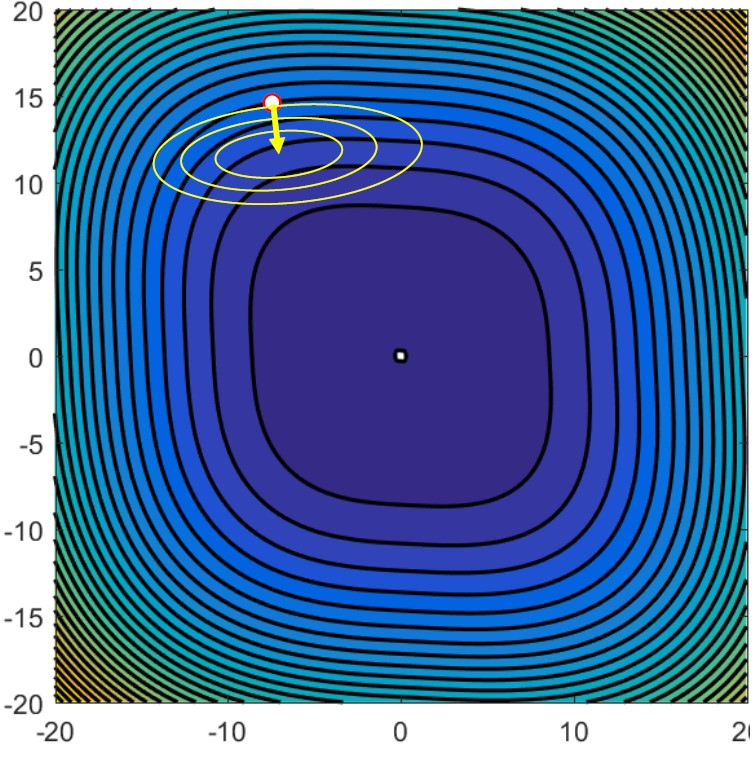
\includegraphics[width=\textwidth]{images/intuition_newton2.jpeg}
        \end{minipage}
    \caption{Fit a quadratic at each point and find the minimum of that quadratic}
    \end{figure}
\end{frame}

\begin{frame}{Newton's Method: The Update Rule}
    \framesubtitle{Incorporating the Hessian}
    The update rule incorporates the \textbf{Hessian matrix ($H$)}, the matrix of second derivatives, which describes the local curvature.
    \begin{itemize}
        \item The update rule is:
            $$ w^{(k+1)} = w^{(k)} - H_{E}(w^{(k)})^{-1} \nabla_{w}E(w^{(k)}) $$
        \item By multiplying the gradient by the \textbf{inverse Hessian}, the update is rescaled. This effectively transforms the elliptical contours of an ill-conditioned problem into circular ones, allowing for a direct path to the minimum.
        \item For a quadratic function, the optimal $\eta$ is 1 (which is exactly Newton's method). Therefore, this method has no learning rate/hyperparameter to tune; the optimal step size is effectively 1.
    \end{itemize}
\end{frame}



\begin{frame}{Visualizing Second-Order Optimization}
    \framesubtitle{The Effect of Preconditioning}
    
    \begin{figure}
        \centering
        % This tikzpicture environment manually places all elements
        \begin{tikzpicture}
            % Define coordinates for the center of each image
            \coordinate (pos1) at (-3.5, 5.5);
            \coordinate (pos2) at (3.5, 5.5);
            \coordinate (pos3) at (-3.5, 2);
            \coordinate (pos4) at (3.5, 2);
            
            % Place the images as nodes at the defined positions
            \node at (pos1) {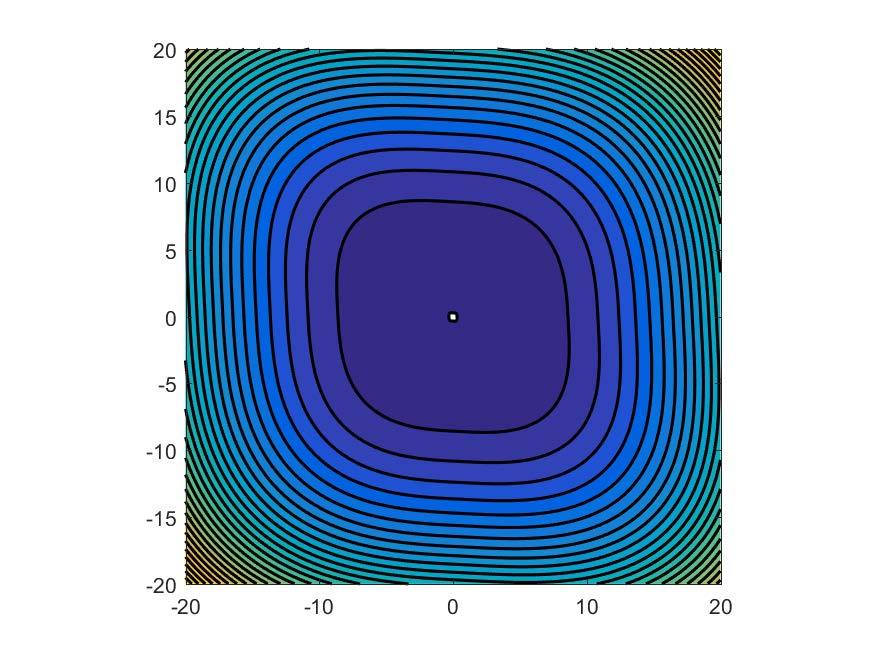
\includegraphics[width=0.4\textwidth]{images/contour_before_seocnd.jpeg}};
            \node at (pos2) {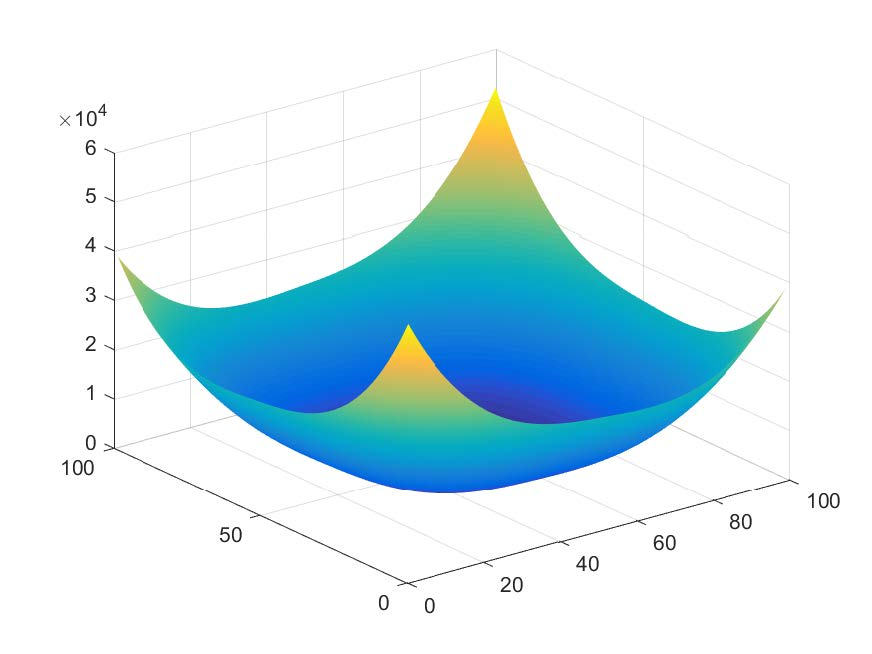
\includegraphics[width=0.4\textwidth]{images/loss_before_second.jpeg}};
            \node at (pos3) {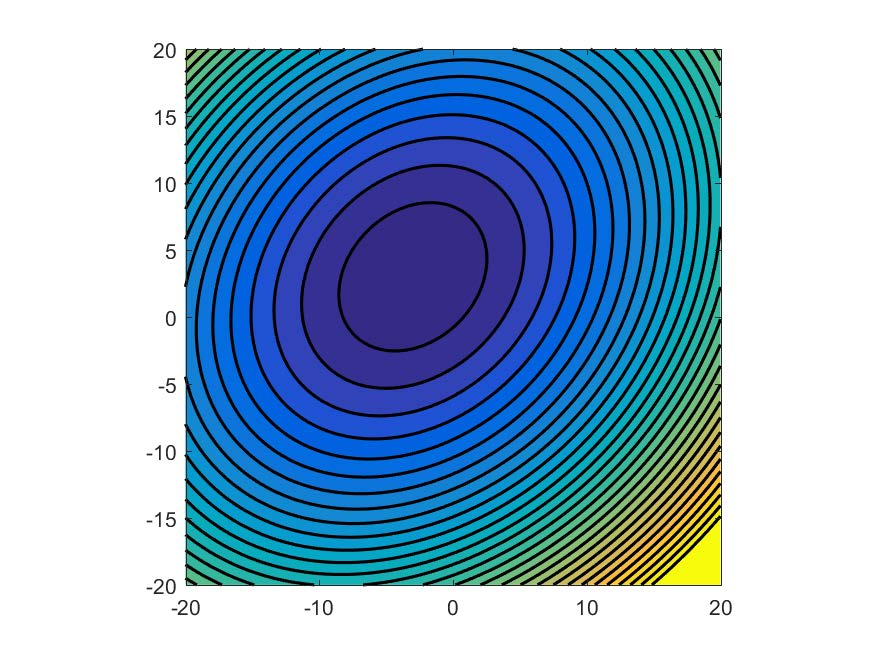
\includegraphics[width=0.4\textwidth]{images/contour_after_second.jpeg}};
            \node at (pos4) {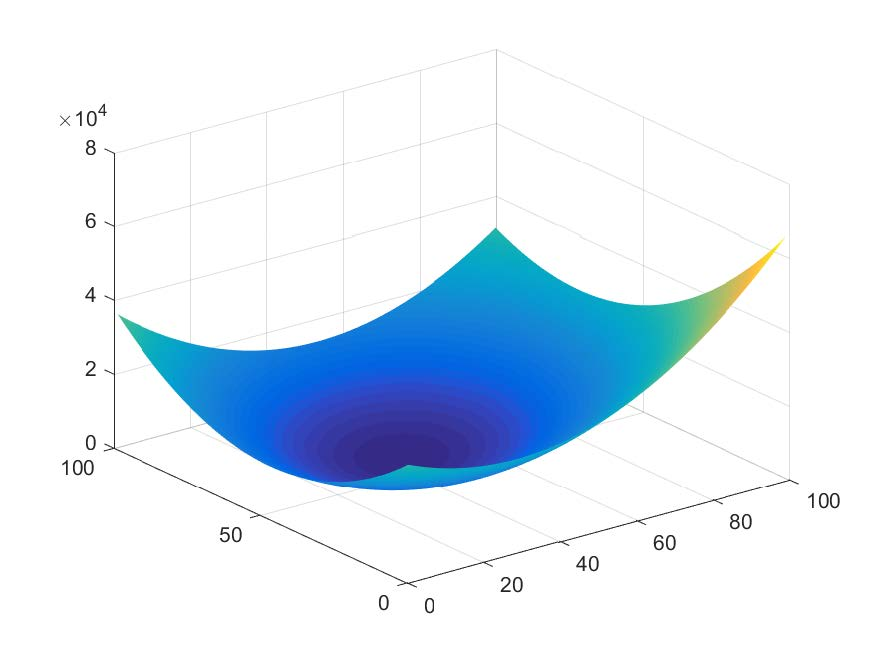
\includegraphics[width=0.4\textwidth]{images/loss_after_second.jpeg}};
            
            % Define the start and end points for the arrow, centered horizontally
            \coordinate (arrow_start) at (0, 5);
            \coordinate (arrow_end) at (0, 3);
            
            % Draw the arrow using the standard -> tip
            \draw[->, ultra thick, blue!60!white, line width=2pt] 
                (arrow_start) -- (arrow_end);
        \end{tikzpicture}
        \caption{Visualizing the error surface before (top) and after (bottom) applying second-order information.}
    \end{figure}
    
\end{frame}





\begin{frame}{The Drawbacks of Newton's Method}
    \framesubtitle{Why It's Impractical for Deep Learning}
    Despite its rapid convergence, Newton's method is not used for large-scale deep learning.
    \begin{itemize}
        \item \textbf{Prohibitive Computational Cost}:
        \begin{itemize}
            \item For a network with $n$ parameters, the Hessian matrix has $n^2$ elements.
            \item Calculating the Hessian takes $O(n^2)$ time.
            \item Inverting it takes $O(n^3)$ time. For millions of parameters, this is infeasible.
        \end{itemize}
        \item \textbf{Stability Issues on Non-Convex Surfaces}:
        \begin{itemize}
            \item For non-convex functions, the Hessian may not be positive definite. This can cause the update to move towards a saddle point or maximum instead of a minimum.
        \end{itemize}
    \end{itemize}
\end{frame}

\begin{frame}{Quasi-Newton Methods: A Practical Compromise}
    \framesubtitle{Approximating the Inverse Hessian}
    \begin{itemize}
        \item \textbf{Quasi-Newton methods}, like BFGS, avoid the full computation of the inverse Hessian.
        \item They iteratively build up an approximation of the inverse Hessian using only first-order gradient information.
        \item \textbf{L-BFGS (Limited-memory BFGS)} is a popular variant that uses only the last few gradient updates, making it more memory-efficient.
        \item However, L-BFGS works best in a full-batch, deterministic setting and does not transfer well to the noisy, mini-batch updates common in deep learning.
    \end{itemize}
    \begin{alertblock}{Next Steps}
        Since second-order methods are too costly, we look for more sophisticated first-order methods that can tackle the conditioning problem without computing the Hessian.
    \end{alertblock}
\end{frame}

\subsection{Momentum Methods}

\begin{frame}{Momentum Methods}
    \frametitle{Accelerating Gradient Descent}
    \begin{itemize}
        \item Momentum methods are designed to accelerate learning, especially in deep, narrow valleys where vanilla gradient descent is slow.
        \item \textbf{The Core Idea:} Keep track of past gradients to build up "velocity" in consistent directions and dampen oscillations in steep directions.
        \item This is analogous to a heavy ball rolling down the error surface; it builds up momentum and is less affected by small bumps and changes in gradient direction.
    \end{itemize}

\end{frame}

\begin{frame}{Momentum Methods}
    \frametitle{Intuition Behind Momentum}
    \begin{figure}
        \centering
        \begin{minipage}{0.5\textwidth}
            \centering
            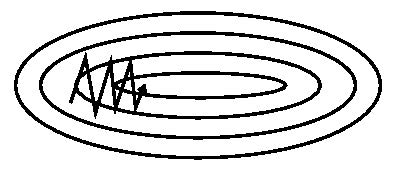
\includegraphics[width=\textwidth]{images/before_momentum.jpeg}
            \captionof{figure}{Plain gradient update}
        \end{minipage}%
            \begin{minipage}{0.5\textwidth}
            \centering
            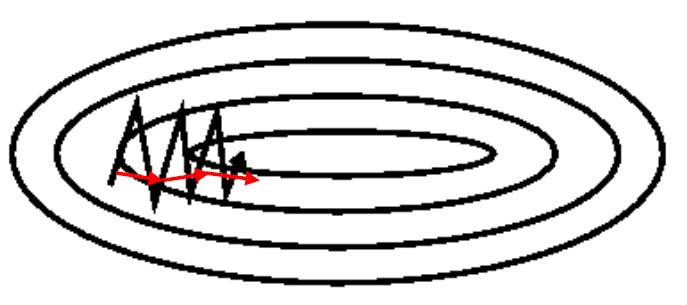
\includegraphics[width=\textwidth]{images/after_momentum.jpg}
            \captionof{figure}{With momentum}
        \end{minipage}
        \caption*{Momentum helps accelerate in consistent directions and dampens oscillations.}
    \end{figure}
\end{frame}

\begin{frame}{Standard Momentum}
    \frametitle{The Momentum Update Rule}
    This method adds a fraction of the previous update vector to the current gradient step.
    \begin{itemize}
        \item A velocity vector, $v$, accumulates an \bhighlight{exponentially decaying moving average} of past gradients.
        \item The update rule is:
            $$ \textcolor{red}{v^{(k)}} = \textcolor{violet}{\beta v^{(k-1)}} + \textcolor{green}{\eta \nabla_w E(W^{(k-1)})} $$
            $$ W^{(k)} = W^{(k-1)} - v^{(k)} $$
        \item $\beta$ is the momentum term, typically set to a value like 0.9 \\ It determines how much of the past velocity is retained.
    \end{itemize}
\end{frame}

\begin{frame}{Nesterov Accelerated Gradient (NAG)}
    \frametitle{A Smarter Momentum}
    Nesterov Accelerated Gradient (NAG) is a slightly different, and often more effective, version of the momentum update.
    \begin{itemize}
        \item \textbf{The Idea:} Instead of calculating the gradient at the current position, NAG "looks ahead" by calculating the gradient at a point where the previous velocity would have taken it.
        \item This allows the optimizer to "correct" its course sooner if the gradient is changing, leading to faster convergence.
        \item The update rule is:
             $$ \textcolor{red}{v^{(k)}} = \textcolor{violet}{\beta v^{(k-1)}} + \textcolor{green}{\eta \nabla_w E(W^{(k-1)} - \beta v^{(k-1)})} $$
             $$ W^{(k)} = W^{(k-1)} - v^{(k)} $$
    \end{itemize}
\end{frame}

\begin{frame}{Visual Comparison: Momentum vs. NAG}
    \frametitle{The "Look-Ahead" Advantage}
    \begin{columns}[T]
        \begin{column}{0.5\textwidth}
            \textbf{Standard Momentum}
            \footnotesize % Using a smaller font for the description
            \begin{enumerate}
                \item Computes gradient at current position.
                \item Adds scaled previous velocity.
            \end{enumerate}
            
            \begin{figure}
                % Placeholder for momentum update diagram from Optimization I.pdf, p. 63
                % Increased width to fill the column
                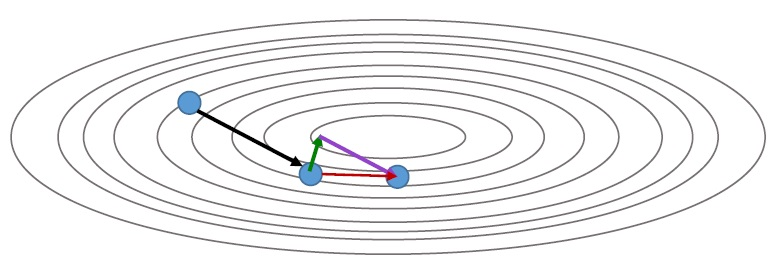
\includegraphics[width=\linewidth]{images/standard_momentum.jpg}
            \end{figure}
        \end{column}
        
        \begin{column}{0.5\textwidth}
            \textbf{NAG}
            \footnotesize % Using a smaller font for the description
            \begin{enumerate}
                \item First, takes a step in direction of previous velocity.
                \item Computes gradient at this "look-ahead" position and makes a correction.
            \end{enumerate}
            
            \begin{figure}
                % Placeholder for NAG update diagram from Optimization I.pdf, p. 70
                % Increased width to fill the column
                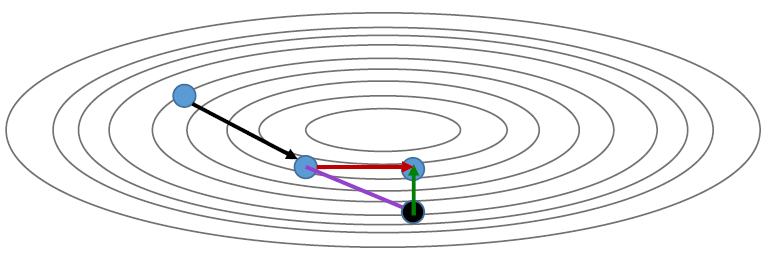
\includegraphics[width=\linewidth]{images/nag.png}
            \end{figure}
        \end{column}
    \end{columns}
    
\end{frame}

\subsection{Adaptive Learning Rate Methods}

\begin{frame}{The Optimizer's Dilemma}
    \framesubtitle{One Learning Rate to Rule Them All?}
    \begin{itemize}
        \item We've seen that Momentum helps us move faster by building velocity.
        \item \textbf{But there's a problem:} It's like driving a car where all four wheels are forced to turn at the same angle. On a winding road (our ill-conditioned error surface), this is clumsy.
        \item Some parameters (wheels) need to turn sharply (small learning rate), while others need to go straight (large learning rate).
        \item \textbf{The Goal:} Give each parameter its own "smart" learning rate that adapts automatically to the terrain it's on.
    \end{itemize}
\end{frame}

\begin{frame}{Adagrad: The Historian}
    \framesubtitle{Every Gradient Leaves a Mark}
    \bhighlight{Adagrad} was a pioneering idea that gave each parameter a personal learning rate.
    \begin{itemize}
        \item \textbf{The Strategy:} Keep a running sum of the squares of all past gradients for each parameter.
        \item Parameters that have seen large gradients in the past will have their learning rate aggressively decreased.
        \item The update rule:
            $$ s^{(k)} = s^{(k-1)} + (\nabla_w E)^2 $$
            $$ W^{(k+1)} = W^{(k)} - \frac{\eta}{\sqrt{s^{(k)} + \epsilon}} \nabla_w E $$
        \item \textbf{The Fatal Flaw:} The denominator, $s^{(k)}$, is a sum that only ever grows, it eventually stops the learning process entirely as the learning rate vanishes.
    \end{itemize}
\end{frame}

\begin{frame}{RMSProp: The Forgetful Historian}
    \framesubtitle{Remembering Only the Recent Past}
    \bhighlight{RMSProp} solves Adagrad's problem by forgetting the distant past and focusing only on recent gradient history.
    \begin{itemize}
        \item Instead of a sum, it uses an \textbf{exponentially decaying moving average} of squared gradients.
        \item This prevents the denominator from growing indefinitely, allowing learning to continue.
        \item The update rule:
            $$ \overline{(\nabla_w E^2)}^{(k)} = \beta \overline{(\nabla_w E^2)}^{(k-1)} + (1-\beta)(\nabla_w E)^2 $$
            $$ W^{(k+1)} = W^{(k)} - \frac{\eta}{\sqrt{\overline{(\nabla_w E^2)}^{(k)} + \epsilon}} \nabla_w E $$
        \item It effectively normalizes each parameter's update by the magnitude of its recent gradients.
    \end{itemize}
\end{frame}

\begin{frame}{Adam: The Best of Both Worlds}
    \framesubtitle{Adaptive Moment Estimation}
    Adam is the most popular optimizer because it combines the best ideas we've seen so far.
    \begin{itemize}
        \item It's a hybrid of \textbf{Momentum} and \textbf{RMSProp}.
        \item It uses a moving average of the gradient itself (like Momentum) to track the direction of travel (the \textit{first moment}).
        \item It uses a moving average of the squared gradient (like RMSProp) to adapt the learning rate for each parameter (the \textit{second moment}).
    \end{itemize}
    \begin{alertblock}{The Result}
        An optimizer that knows both where it's going and how fast it should get there, for every single parameter.
    \end{alertblock}
\end{frame}

\begin{frame}{The Adam Update Rule}
    \framesubtitle{Putting It All Together}
    \small
    Adam maintains two moving averages, $m$ (for momentum) and $v$ (for variance scaling), and includes a bias-correction step.
    \begin{enumerate}
        \item First moment (Momentum):
            $$ m^{(k)} = \beta_1 m^{(k-1)} + (1-\beta_1) g^{(k)} $$
        \item Second moment (RMSProp):
            $$ v^{(k)} = \beta_2 v^{(k-1)} + (1-\beta_2) (g^{(k)})^2 $$
        \item Bias Correction (to counteract initialization at zero):
            $$ \hat{m}^{(k)} = \frac{m^{(k)}}{1 - \beta_1^k} \quad , \quad \hat{v}^{(k)} = \frac{v^{(k)}}{1 - \beta_2^k} $$
        \item Final Update Rule:
            $$ W^{(k+1)} = W^{(k)} - \frac{\eta}{\sqrt{\hat{v}^{(k)} + \epsilon}} \hat{m}^{(k)} $$
    \end{enumerate}
    \footnotesize{Common hyperparameters: $\eta$ (needs tuning), $\beta_1=0.9$, $\beta_2=0.999$, $\epsilon=10^{-8}$.}
\end{frame}

\begin{frame}{The Problem of Bias in Adam}
    \framesubtitle{The "Cold Start" Problem}
    \begin{itemize}
        \item Adam's moment vectors, $m$ and $v$, are initialized to zero.
        \item In the first few iterations, the moving averages are heavily weighted by these initial zeros, making them biased towards zero.
        \item This "cold start" causes the optimizer to take very small steps at the beginning of training, when it should be making the most progress.
    \end{itemize}
    \begin{alertblock}{The Solution: Bias Correction}
        The bias correction step divides the moment estimates by a factor that is initially small and approaches 1 over time. This scales up the early, biased estimates, giving the optimizer a "warm start" and allowing it to take meaningful steps from the very beginning.
    \end{alertblock}
\end{frame}

\begin{frame}{A Word of Caution}
    \framesubtitle{Is Newer Always Better?}
    \begin{itemize}
        \item While Adam is a fantastic default, it's not a silver bullet.
        \item Recent research has shown that adaptive methods can sometimes converge to "sharper" minima that generalize more poorly than the "flatter" minima found by well-tuned \bhighlight{SGD with Momentum}.
        \item There is no single optimizer that dominates across all possible problems.
        \item \textbf{The Takeaway:} Adam is a great starting point, but if you're aiming for state-of-the-art results, it can be worth trying to carefully tune SGD+Momentum as well.
    \end{itemize}
\end{frame}

\begin{frame}{Working with Data}
    \framesubtitle{The Problem with Full-Batch Updates}
    \begin{itemize}
        \item In standard (or "batch") gradient descent, we compute the gradient of the cost function using the \bhighlight{entire training dataset} for a single update step.
        \[ \nabla_{w}E(W) = \frac{1}{N} \sum_{n=1}^{N} \nabla_{w}\text{loss}(f(x^{(n)}; W), y^{(n)}) \]
        \item \textbf{The Problem:} For modern datasets with millions of examples, this is extremely slow. We have to process all data just to make one small step.
    \end{itemize}
    \begin{figure}
        \centering
        % Source: Optimization II.pdf, Page: 11
        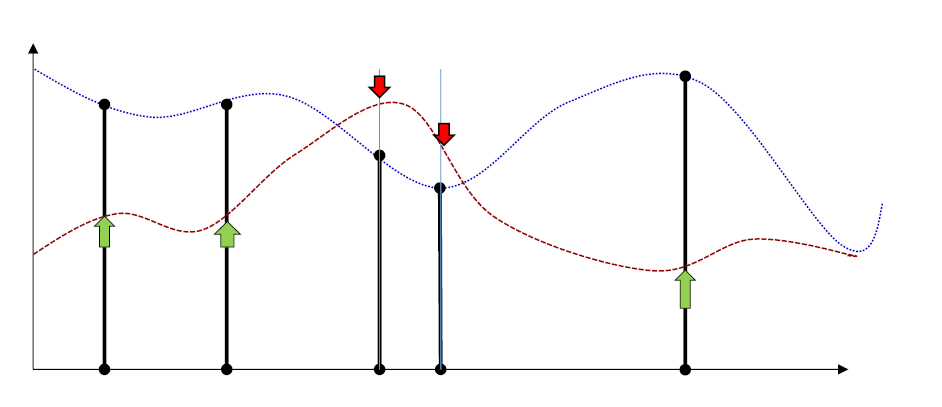
\includegraphics[width=0.7\linewidth]{images/full_batch_idea.png}
        \caption{In batch gradient descent, the algorithm tries to adjust the model based on all training points simultaneously.}
    \end{figure}
\end{frame}

\begin{frame}{Stochastic Gradient Descent (SGD)}
    \framesubtitle{Updating One Sample at a Time}
    \begin{itemize}
        \item The other extreme is \bhighlight{Stochastic Gradient Descent (SGD)}, where we update the weights after seeing \emph{only one} training example at a time.
        \item This makes each update much faster, allowing us to make many more updates in the same amount of time.
    \end{itemize}
    \begin{figure}
        \centering
        % Source: Optimization II.pdf, Page: 15
        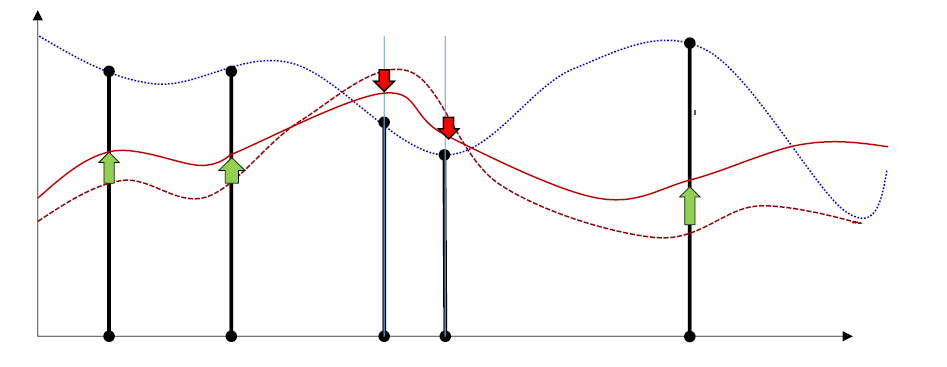
\includegraphics[width=0.7\linewidth]{images/sgd_step_1.png}
        \caption{With SGD, the function is first adjusted for a single, random training point...}
    \end{figure}
\end{frame}

\begin{frame}{Stochastic Gradient Descent (SGD)}
    \framesubtitle{Iterating Through Samples}
    \begin{figure}
        \centering
        % Source: Optimization II.pdf, Page: 16
        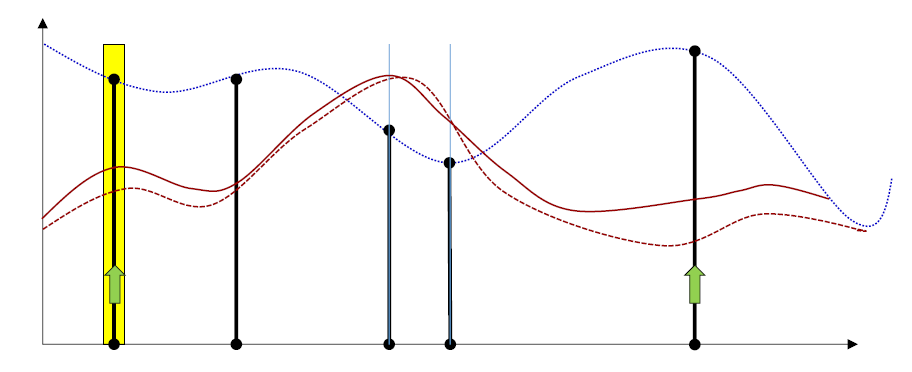
\includegraphics[width=0.7\linewidth]{images/sgd_step_2.png}
        \caption{...then it is adjusted for the next random point...}
    \end{figure}
\end{frame}

\begin{frame}{Stochastic Gradient Descent (SGD)}
    \framesubtitle{Completing an Epoch}
    \begin{figure}
        \centering
        % Source: Optimization II.pdf, Page: 17
        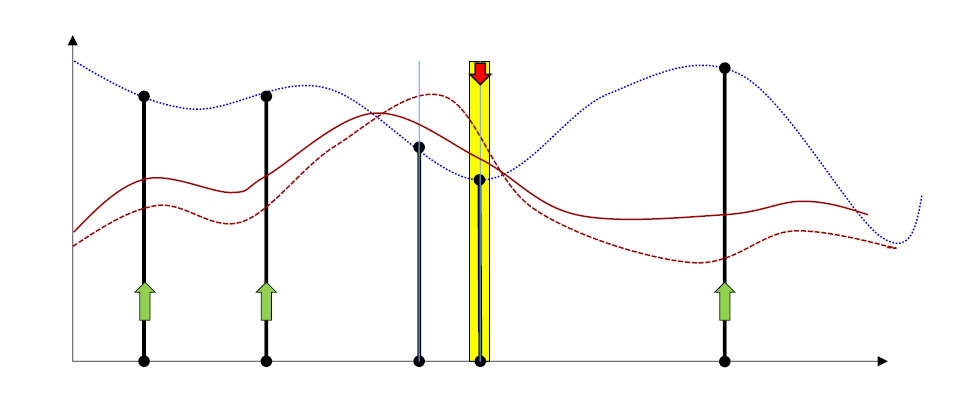
\includegraphics[width=0.7\linewidth]{images/sgd_step_3.png}
        \caption{...and so on. After passing through all points once (an epoch), the entire function has been adjusted.}
    \end{figure}
\end{frame}

\begin{frame}{Stochastic Gradient Descent (SGD)}
    \framesubtitle{The Algorithm and Key Concepts}
    \begin{itemize}
        \item \textbf{The Update Rule:} For a single sample $(x^{(n)}, y^{(n)})$:
        \[ w^{t+1} = w^{t} - \eta \nabla_{w}\text{loss}(f(x^{(n)}; W), y^{(n)}) \]
        \item \textbf{Epoch:} A single full pass through the entire training dataset is called an \bhighlight{epoch}. In one epoch of SGD, we make N weight updates.
        \item \textbf{Crucial Requirement:} For SGD to work correctly, the training data must be \bhighlight{shuffled} at the beginning of every epoch. This randomness is essential for good convergence.
    \end{itemize}
\end{frame}

\begin{frame}{Stochastic Gradient Descent (SGD)}
    \framesubtitle{The "Stochastic" Nature}
    \begin{itemize}
        \item The gradient from a single sample is a "noisy" but \bhighlight{unbiased estimate} of the true gradient over the full dataset.
        \item This high variance means the path to the minimum is erratic and jittery. The updates may not always move towards the minimum and can sometimes move away from it.
    \end{itemize}
    \begin{figure}
        \centering
        % Source: Optimization I.pdf, Page: 9
        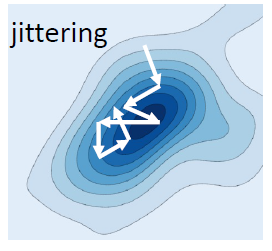
\includegraphics[width=0.2\linewidth]{images/convergence_behaviors.png}
        \caption{The path of SGD often resembles the "jittering" behavior, where it oscillates around the minimum without perfectly converging.}
    \end{figure}
\end{frame}

\begin{frame}{Stochastic Gradient Descent (SGD)}
    \framesubtitle{The Need for Learning Rate Annealing}
    \begin{itemize}
        \item Because the gradient is always noisy, the updates will never settle at the exact minimum if the learning rate $\eta$ remains constant. The optimization will just jitter around it indefinitely.
        \item To ensure convergence, the learning rate must be \bhighlight{decayed over time}. This is called \bhighlight{learning rate annealing} or scheduling.
        \item A common strategy is to start with a relatively high learning rate for fast initial progress and gradually reduce it to allow for fine-tuning near the minimum.
    \end{itemize}
\end{frame}

\begin{frame}{Mini-Batch Gradient Descent}
    \framesubtitle{The Best of Both Worlds}
    \begin{itemize}
        \item \bhighlight{Mini-Batch Gradient Descent} is the standard method used in practice. It's a compromise between the full-batch and SGD approaches.
        \item We compute the gradient on a small, random subset of the data called a \bhighlight{mini-batch}.
    \end{itemize}
    \begin{figure}
        \centering
        % Source: Optimization II.pdf, Page: 24
        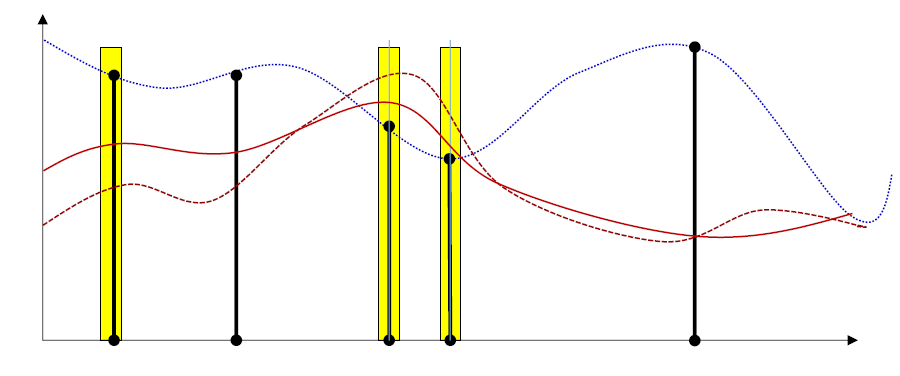
\includegraphics[width=0.7\linewidth]{images/minibatch_idea.png}
        \caption{In Mini-Batch GD, we update the model based on a small, random subset of the data.}
    \end{figure}
\end{frame}

\begin{frame}{Mini-Batch Gradient Descent}
    \framesubtitle{Advantages}
    \begin{itemize}
        \item \textbf{Efficiency:} It allows us to take advantage of the massive parallelization capabilities of GPUs. Matrix operations on a mini-batch are much more efficient than processing samples one by one.
        \item \textbf{Stability:} By averaging gradients over a small batch, we reduce the variance of the updates, leading to a more stable convergence than pure SGD. The path towards the minimum is less erratic.
    \end{itemize}
\end{frame}

\begin{frame}{Comparing the Update Strategies}
    \framesubtitle{A Visual Guide}
    \begin{figure}
        \centering
        % Source: Optimization II.pdf, Page: 47
        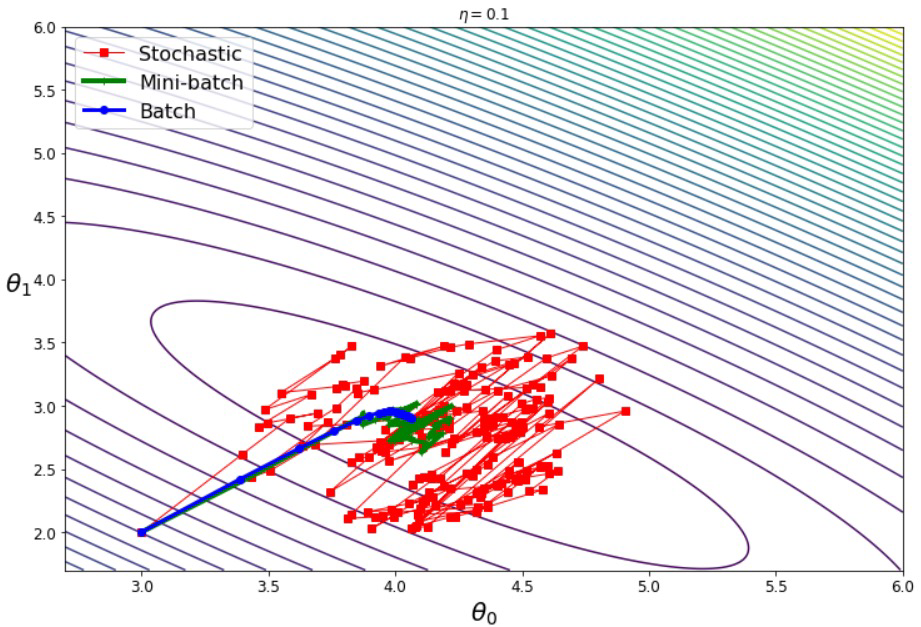
\includegraphics[width=0.9\linewidth]{images/optimizer_paths.png}
        \caption{
            \textbf{Batch (Blue):} Takes a smooth, direct path but each step is very slow.
            \textbf{Stochastic (Red):} Very noisy and erratic path, but takes many fast steps.
            \textbf{Mini-Batch (Green):} A good balance, reducing noise while still being computationally efficient.
        }
    \end{figure}
\end{frame}

\begin{frame}{Choosing the Mini-Batch Size}
    \framesubtitle{A Practical Guideline}
    \begin{itemize}
        \item The mini-batch size is a hyperparameter that needs to be chosen.
        \item If the training set is very small (e.g., < 2000 examples), you can often use full-batch gradient descent.
        \item For larger datasets, typical mini-batch sizes are powers of 2, such as \bhighlight{32, 64, 128, 256, 512}.
        \item A key constraint is that the mini-batch of data and the resulting gradients must fit into your GPU's memory.
    \end{itemize}
\end{frame}

\section{Generalization}

\subsection{Explicit Regularization}

\begin{frame}{The Problem: A Model That Memorizes}
    \frametitle{Overfitting and the Failure to Generalize}
    \begin{itemize}
        \item A model that performs perfectly on training data but fails on new, unseen data has \textbf{overfitted}.
        \item It's like a student who memorizes the answers to past exams but hasn't learned the underlying concepts.
        \item This "generalization gap" is what we aim to reduce.
    \end{itemize}
    \begin{figure}
        % Placeholder for the overfitting graph from Regularization.pdf, p. 5
        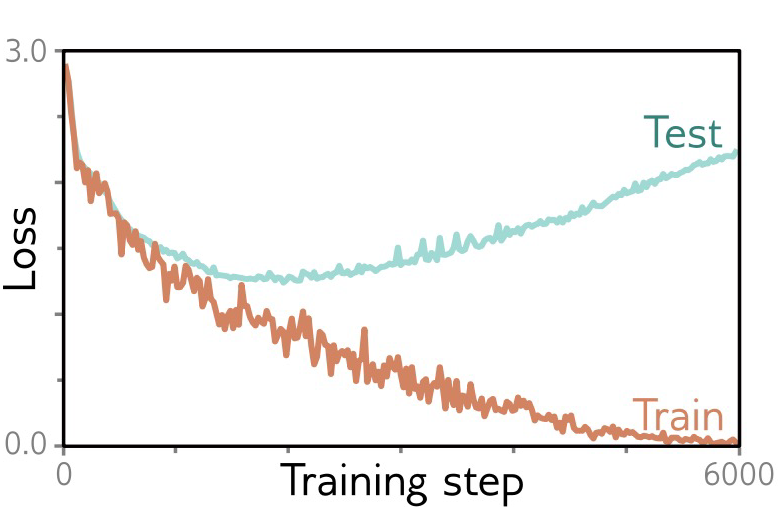
\includegraphics[width=0.7\textwidth]{images/generalization_gap.png}
        \caption{A classic sign of overfitting: training error continues to decrease while test (validation) error begins to rise.}
    \end{figure}
\end{frame}

\begin{frame}{The Solution: A Penalty for Complexity}
    \frametitle{Introducing Regularization}
    How do we encourage our model to learn the true underlying pattern instead of just memorizing the data points?
    \begin{itemize}
        \item We can add a \bhighlight{penalty term} $R(W)$ to our loss function.
        \item This penalty discourages the model from becoming too complex.
        \item Our new objective is to balance two competing goals:
            \begin{enumerate}
                \item Fit the training data well (minimize the original loss).
                \item Keep the model simple (minimize the regularization penalty).
            \end{enumerate}
        \item The new cost function is:
            $$ J(W) = \underbrace{\sum_{n=1}^{N}\text{loss}(y^{(n)}, f(x^{(n)}; W))}_{\text{Data Fit}} + \underbrace{\lambda R(W)}_{\text{Complexity Penalty}} $$
    \end{itemize}
\end{frame}

\begin{frame}{L2 Regularization (Weight Decay)}
    \frametitle{L2 Regularization (Weight Decay)}
    L2 regularization penalizes the squared magnitude of the weights. It encourages the network to use small weights.
    \begin{itemize}
        \item The penalty term is the squared L2 norm of the weights:
            $$ R(W) = ||W||_2^2 = \sum_k \sum_l W_{k,l}^2 $$
        \item The new cost function becomes:
            $$ J(W) = \text{Loss}(W) + \lambda ||W||_2^2 $$
        \item This leads to a modified gradient update rule called \textbf{Weight Decay}:
            $$ W \leftarrow W - \alpha \nabla_W \text{Loss}(W) - 2\lambda W $$
            $$ W \leftarrow (1 - 2\lambda)W - \alpha \nabla_W \text{Loss}(W) $$
        \item At each step, the weights are multiplicatively shrunk before the gradient update.
    \end{itemize}
\end{frame}

\begin{frame}{The Intuition Behind L2 Regularization}
    \frametitle{Why Do Smaller Weights Generalize Better?}
    \begin{itemize}
        \item \textbf{Smoother Functions:} Penalizing large weights forces the network to learn smoother, less complex functions.
        \item \textbf{Linear Regime:} With tanh or sigmoid activations, small weights keep neurons in their linear range. Since linear neurons can only learn simple linear functions, L2 regularization promotes this low-complexity behavior.
    \end{itemize}
    \begin{figure}
        % Placeholder for the sigmoid visualization from Regularization.pdf, p. 14
        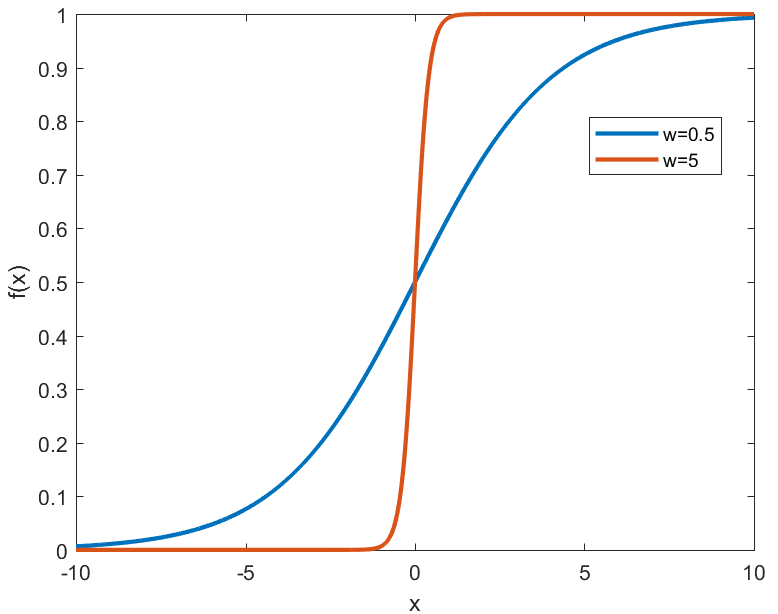
\includegraphics[width=0.5\textwidth]{images/sigmoid_l2.png}
        \caption{As weight `w` increases, the sigmoid function becomes much steeper and more non-linear, allowing for more complex responses.}
    \end{figure}
\end{frame}

\begin{frame}{The Effect of the Regularization Strength $\lambda$}
    \frametitle{Finding the Right Balance}
    The hyperparameter $\lambda$ controls the trade-off between fitting the data and keeping the weights small.
    \begin{figure}
        % Placeholder for the lambda effect visualization from Regularization.pdf, p. 11
        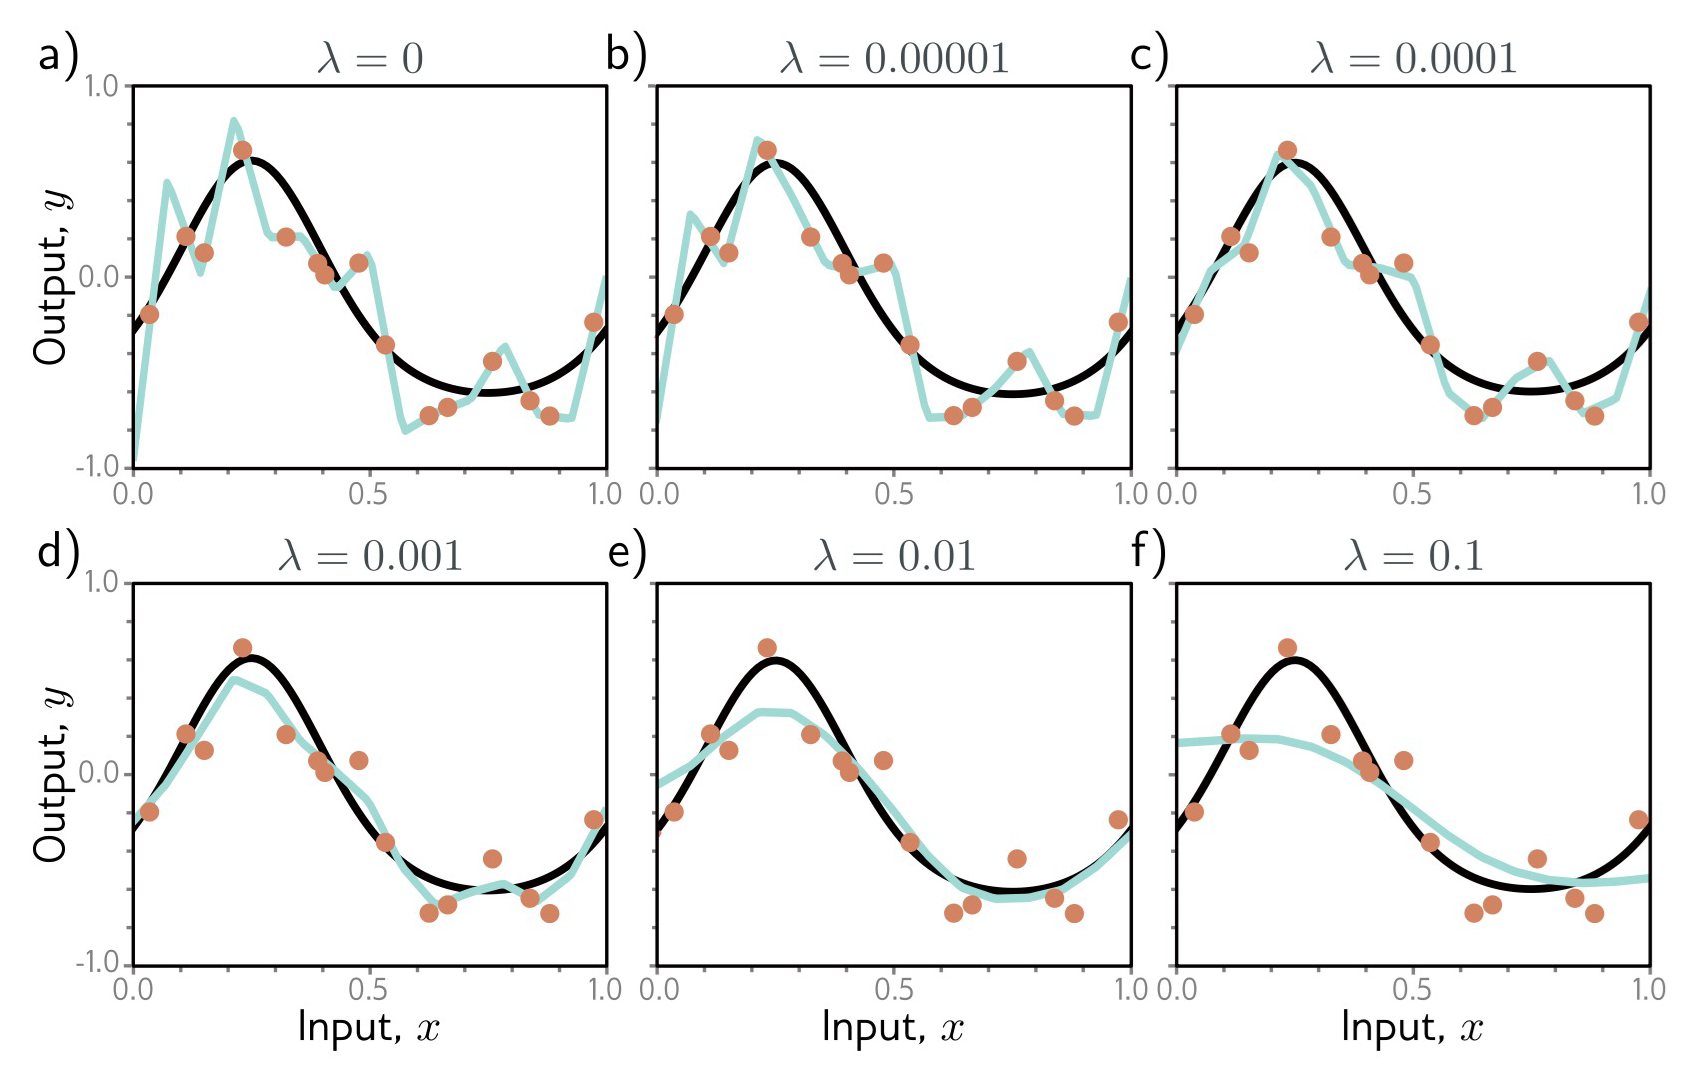
\includegraphics[width=0.9\textwidth]{images/lambda_effect.png}
        \caption{As $\lambda$ increases, the learned function becomes smoother and less prone to overfitting, but too high a value can lead to underfitting.}
    \end{figure}
\end{frame}

\begin{frame}{Geometric Intuition of regularizations}
    L1 regularization penalizes the absolute value of the weights.
    \begin{itemize}
        \item The penalty term is the L1 norm of the weights:
            $$ R(W) = ||W||_1 = \sum_k \sum_l |W_{k,l}| $$
        \item \textbf{Key Property:} L1 regularization is known for producing \bhighlight{sparse weight} vectors. It encourages many weights to be exactly zero.
        \item This can be interpreted as a form of automatic feature selection, as the network learns to ignore irrelevant inputs.
    \end{itemize}
    \begin{alertblock}{L1 vs. L2}
        Use L2 regularization as a default. L1 can be useful if you suspect many of your input features are irrelevant and you want a sparse, more interpretable model.
    \end{alertblock}
\end{frame}

\begin{frame}{Geometric intuition of regularizations}
    \begin{columns}
        \begin{column}{0.5\textwidth}
            \textbf{L2 Regularization}
            \begin{itemize}
                \item Circular constraint
                \item Smooth shrinkage
            \end{itemize}
        \end{column}
        \begin{column}{0.5\textwidth}
            \textbf{L1 Regularization}
            \begin{itemize}
                \item Diamond constraint
                \item Corners hit first
            \end{itemize}
        \end{column}
    \end{columns}

    \vspace{1em}

    \begin{figure}
        \centering
        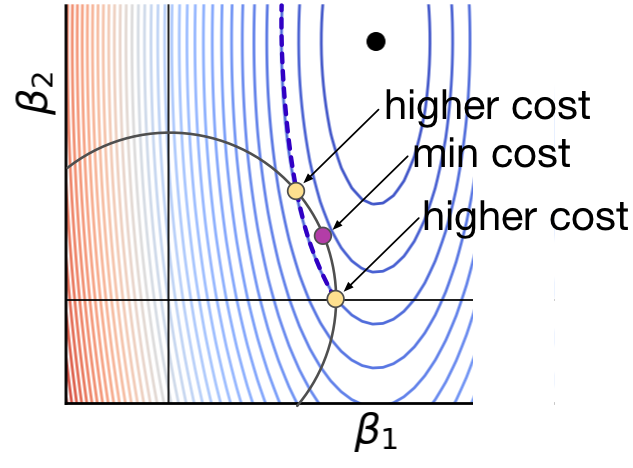
\includegraphics[width=0.45\textwidth]{images/L2contour.png}
        \hspace{1em}
        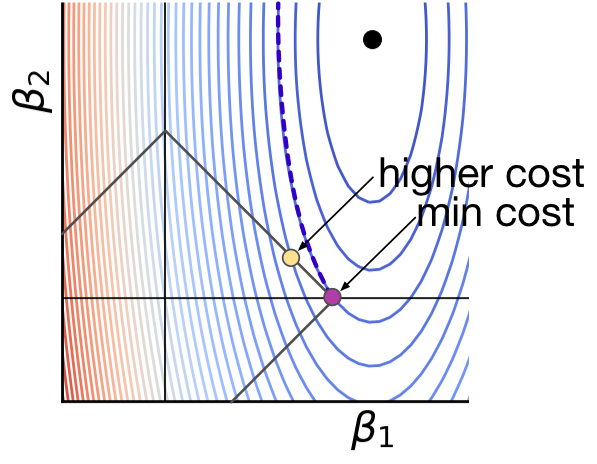
\includegraphics[width=0.45\textwidth]{images/L1contour.png}
        \caption{L1 and L2 constraint regions get different coefficient locations, on the diamond and circle, for the same loss function. Keep in mind that there are an infinite number of contour lines and there is a contour line exactly meeting the L2 purple dot.}
    \end{figure}
\end{frame}

\begin{frame}{Elastic Net: The Best of Both Worlds}
    What if you want both sparsity from L1 and the smoothing effect of L2?
    \begin{itemize}
        \item \bhighlight{Elastic Net} regularization is a hybrid approach that combines both L1 and L2 penalties.
        \item The penalty term is a simple weighted sum of the L1 and L2 norms:
            $$ R(W) = \sum_k \sum_l \beta W_{k,l}^2 + |W_{k,l}| $$
        \item It can produce sparse models like L1.
        \item It is more stable and often performs better than L1 when features are highly correlated.
    \end{itemize}
\end{frame}

\begin{frame}{Regularization: Dropout}
    \framesubtitle{A Simple and Powerful Idea}
    \small
    \begin{itemize}
        \item \bhighlight{Dropout} is a regularization technique that prevents complex co-adaptations on training data by randomly dropping units (along with their connections) from the neural network during training.
        \item \textbf{The Core Idea:} In each forward pass, for each training example, we randomly set the output of some neurons to zero.
        \item The probability of keeping a neuron active is a hyperparameter, often set to 0.5.
    \end{itemize}
    \begin{figure}
        \centering
        % Source: Regularization.pdf, Page: 24
        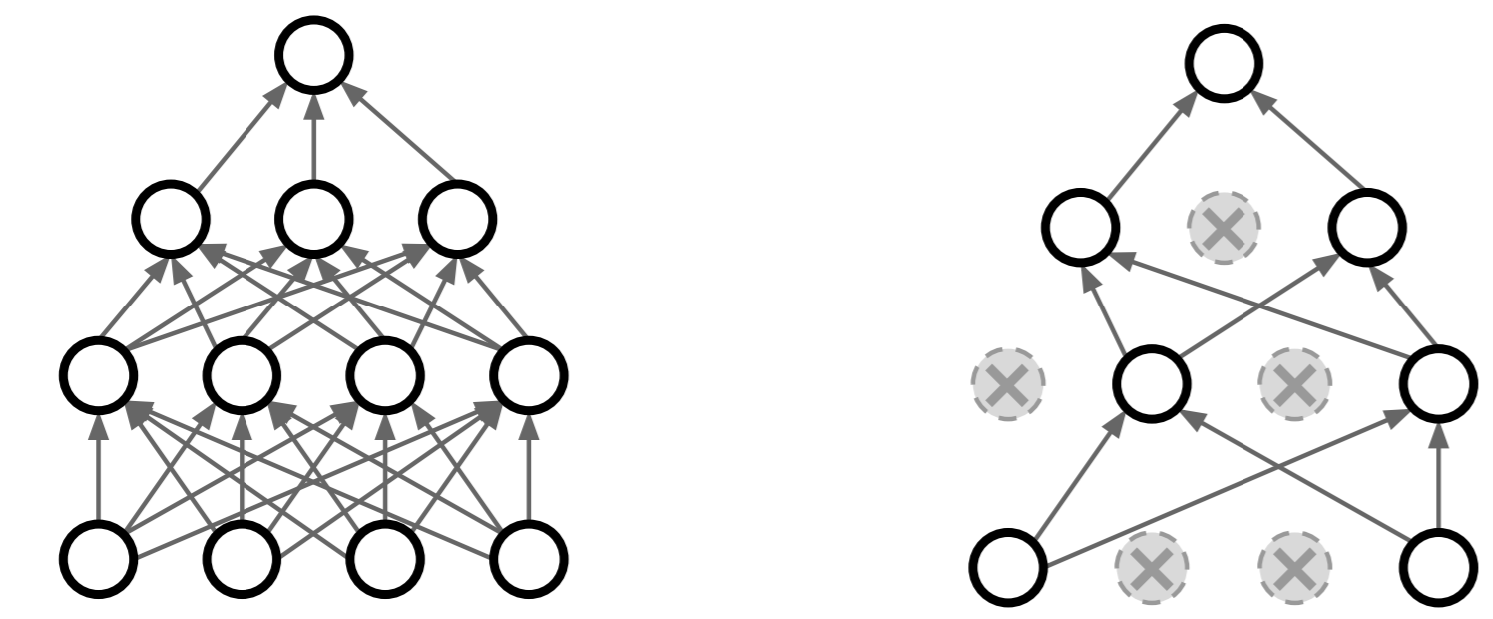
\includegraphics[width=0.7\linewidth]{images/dropout_idea.png}
        \caption{Left: A standard neural network. Right: The same network after applying dropout. Some neurons are temporarily deactivated.}
    \end{figure}
\end{frame}

\begin{frame}{Dropout: The Training Process}
    \framesubtitle{Training a Thinned Network}
    \small
    \begin{itemize}
        \item During each training step, we are effectively training a different, "thinned" version of the network for each mini-batch.
        \item The backpropagation step only updates the weights of the "active" neurons and connections for that specific forward pass.
        \item This forces the network to learn more robust and redundant features, as it cannot rely on any single neuron to be present.
    \end{itemize}
    \begin{figure}
        \centering
        % Source: Regularization.pdf, Page: 31
        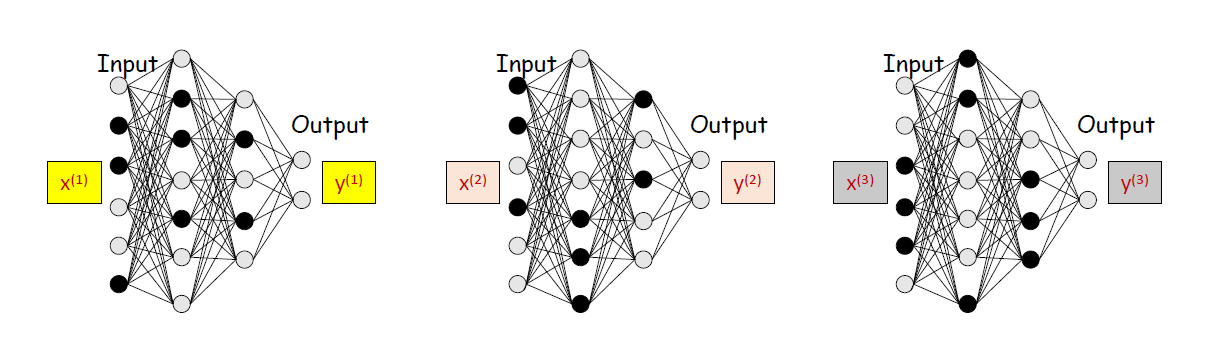
\includegraphics[width=\linewidth]{images/dropout_training_process.png}
        \caption{For each training example, a different random subset of neurons is deactivated, creating a unique "thinned" network.}
    \end{figure}
\end{frame}

\begin{frame}{Why Does Dropout Work?}
    \framesubtitle{Intuition 1: Preventing Co-adaptation}
    \small 
    \begin{itemize}
        \item Dropout prevents neurons from \bhighlight{co-adapting} too much.
        \item A neuron cannot rely on the presence of other specific neurons to correct its mistakes, because those other neurons might be dropped out at any time.
        \item Therefore, each neuron is forced to learn features that are useful on their own, leading to more robust and independent representations.
    \end{itemize}
    \begin{figure}
        \centering
        % Source: Regularization.pdf, Page: 29
        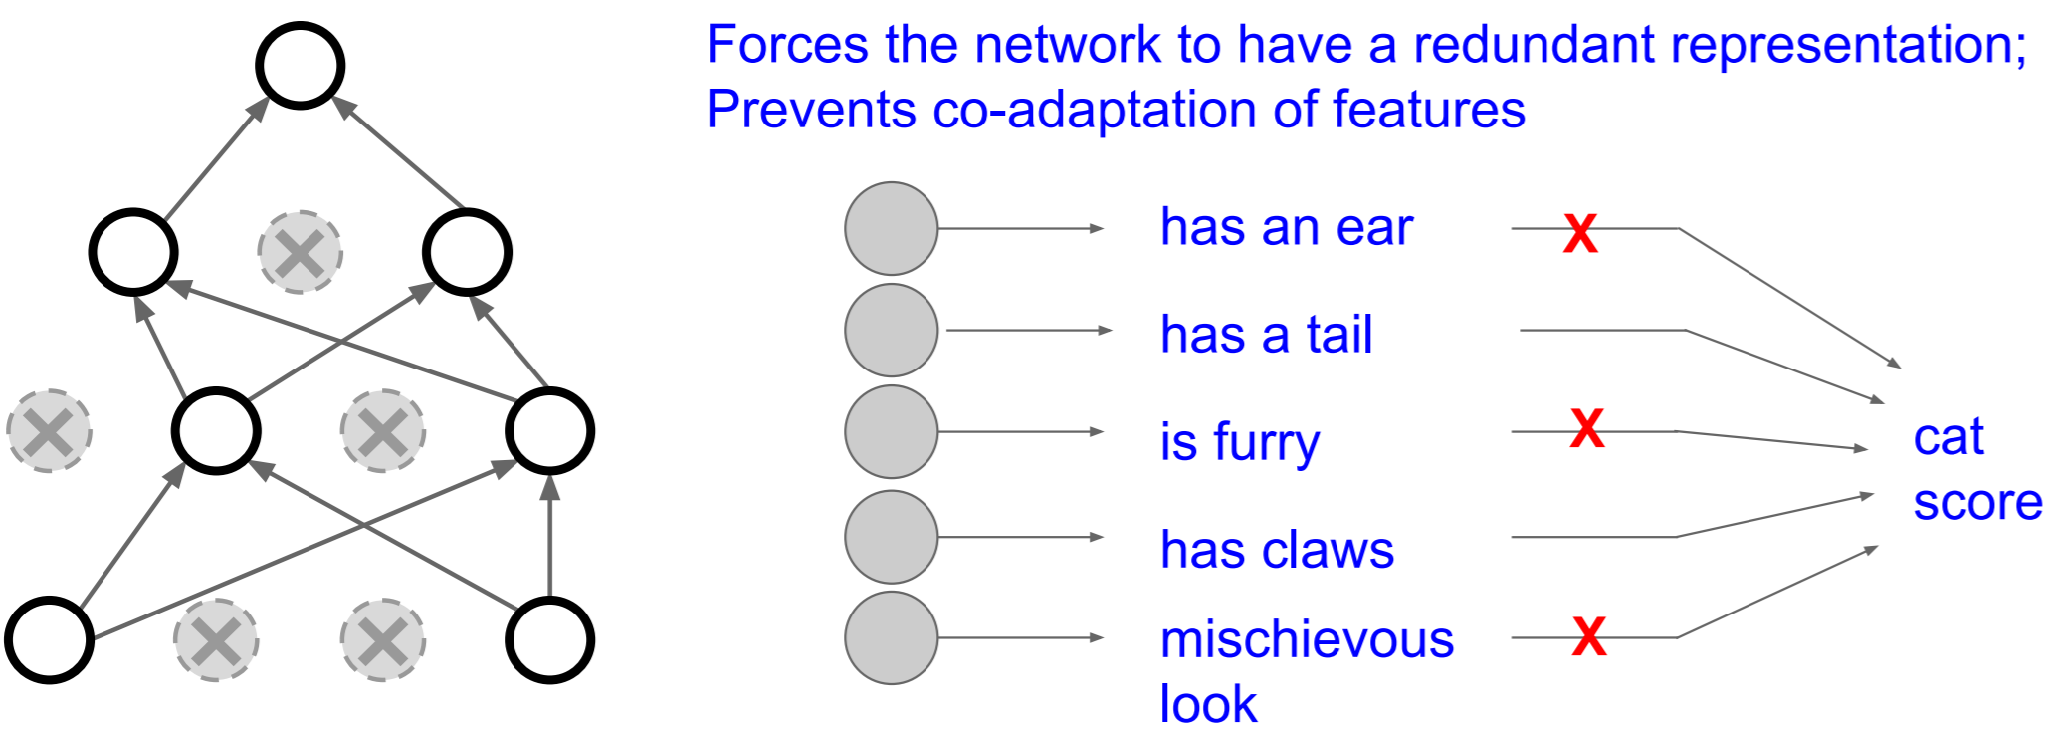
\includegraphics[width=0.8\linewidth]{images/dropout_coadaptation.png}
        \caption{Without dropout, a neuron might learn to rely on a specific feature (e.g., "has whiskers"). With dropout, it must learn from a more diverse set of features.}
    \end{figure}
\end{frame}

\begin{frame}{Why Does Dropout Work?}
    \framesubtitle{Intuition 2: An Ensemble of Networks}
    \small 
    \begin{itemize}
        \item Dropout can be viewed as an efficient way of training a huge \bhighlight{ensemble} of different neural networks.
        \item Each time we randomly drop out neurons, we are essentially training a different network architecture. For a network with N neurons, there are $2^N$ possible thinned networks!
        \item All these networks share weights, so we are effectively training an exponentially large number of models in parallel. At test time, we want to average their predictions.
    \end{itemize}
    \begin{figure}
        \centering
        % Source: Regularization.pdf, Page: 34
        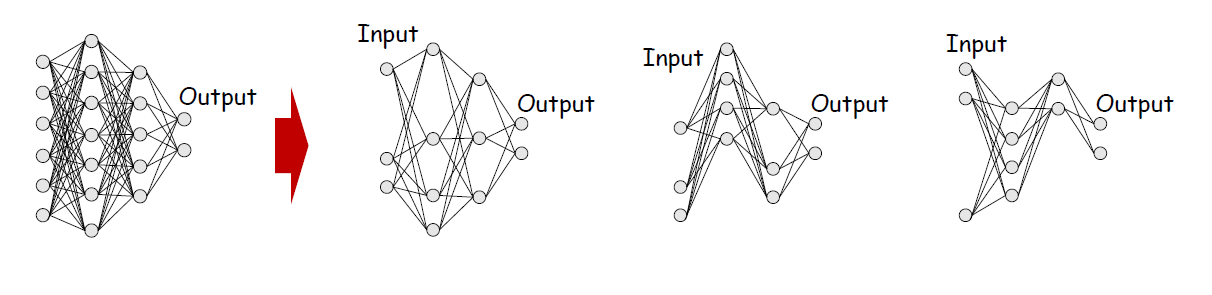
\includegraphics[width=\linewidth]{images/dropout_ensemble.png}
        \caption{Each dropout mask corresponds to training a different sub-network, but they all share the same underlying weights.}
    \end{figure}
\end{frame}

% --- SLIDE WITH CORRECTION ---
\begin{frame}{Dropout at Test Time}
    \framesubtitle{The Problem of Randomness}
    \begin{itemize}
        \item We cannot have random outputs at test time. We need a single, deterministic prediction.
        \item The ideal solution would be to average the predictions of all $2^N$ possible sub-networks, but this is computationally impossible.
        \item \textbf{A Simple Solution:} At test time, we use the full network with all neurons active, but we \bhighlight{scale down the weights} by the probability $p$ (the keep probability) that a neuron was active during training.
        \[ W_{\text{test}} = p \times W_{\text{train}} \]
    \end{itemize}
\end{frame}

\begin{frame}{Inverted Dropout}
    \framesubtitle{A More Common Implementation}
    \begin{itemize}
        \item A more common and practical method is \bhighlight{Inverted Dropout}.
        \item The key idea is to perform the scaling during \bhighlight{training time} instead of test time.
        \item During the forward pass of training, after dropping neurons, the activations of the remaining neurons are immediately scaled up by dividing by the keep probability $p$.
        \[ a^{[l]}_{\text{train}} = \frac{a^{[l]}_{\text{train}} * \text{mask}}{p} \]
        \item \textbf{Advantage:} The forward pass at test time remains completely unchanged. We don't need to do any extra scaling or modifications. This is much cleaner to implement.
    \end{itemize}
\end{frame}

\begin{frame}{Dropout: Practical Considerations}
    \framesubtitle{Tips and Trade-offs}
    \begin{itemize}
        \item \textbf{When to use it:} If your network is significantly overfitting, Dropout is a very effective regularizer.
        \item \textbf{Training Time:} Training with dropout typically takes longer to converge because the gradient updates are noisier and each neuron is trained less often.
        \item \textbf{Dropout Strength:} The keep probability $p$ (often between 0.5 and 0.8) is a hyperparameter you need to tune. A lower $p$ means stronger regularization.
        \item \textbf{Interaction with Batch Norm:} Some evidence suggests that Batch Normalization can reduce the need for Dropout. Using both might not always provide additional benefits.
    \end{itemize}
\end{frame}

\begin{frame}{Dropout: Typical Results}
    \framesubtitle{Impact on Generalization}
    \begin{figure}
        \centering
        % Source: Regularization.pdf, Page: 47
        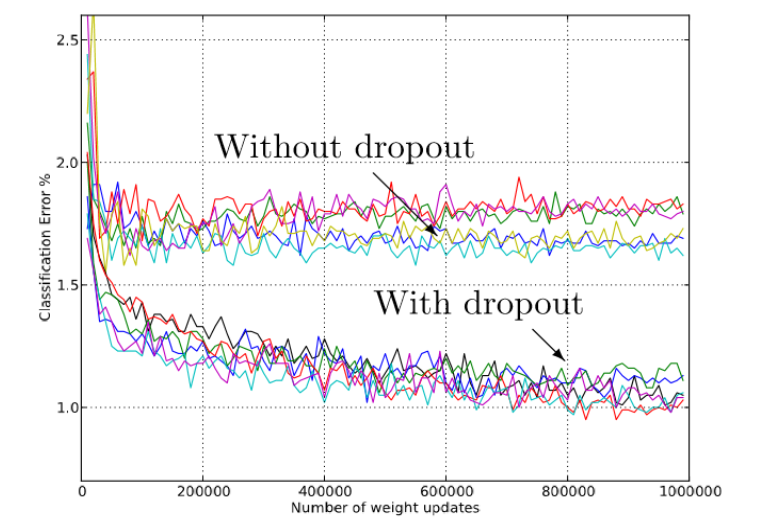
\includegraphics[width=0.9\linewidth]{images/dropout_results.png}
        \caption{A typical result showing that a network trained \textbf{with dropout} (bottom curves) achieves a lower classification error on the test set compared to the same network trained \textbf{without dropout} (top curves).}
    \end{figure}
\end{frame}

\begin{frame}{Generalization: Data Augmentation}
    \framesubtitle{The Best Regularizer: More Data}
    \begin{itemize}
        \item One of the most effective ways to improve a model's generalization is simply to train it on more data.
        \item However, collecting and labeling new data can be expensive and time-consuming.
        \item \bhighlight{Data Augmentation} is a powerful technique to artificially expand the training dataset by creating modified, yet realistic, copies of existing data.
    \end{itemize}
\end{frame}

\begin{frame}{Data Augmentation}
    \framesubtitle{The Core Idea}
    \begin{itemize}
        \item The core idea is to apply transformations to an input example in a way that \bhighlight{does not change its label}.
        \item For example, a horizontally flipped image of a cat is still an image of a cat.
        \item This teaches the model to become \bhighlight{invariant} to these transformations, helping it focus on the true underlying features of the class rather than irrelevant variations in the input.
    \end{itemize}
\end{frame}

\begin{frame}{Data Augmentation}
    \framesubtitle{Examples for Image Data}
    \begin{figure}
        \centering
        % Source: Regularization.pdf, Page: 49
        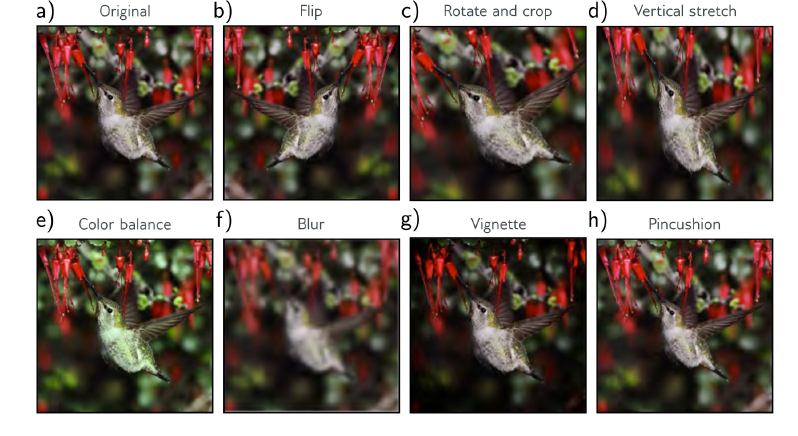
\includegraphics[width=\linewidth]{images/data_augmentation_examples.png}
        \caption{Common augmentation techniques for images include flipping, rotating, cropping, color shifting, blurring, and adding distortions.}
    \end{figure}
\end{frame}

\begin{frame}{Data Augmentation}
    \framesubtitle{Another Technique: Adding Noise}
    \begin{itemize}
        \item Another form of data augmentation is to add random noise directly to the input data.
        \item This can make the model more robust and less sensitive to small variations in the input, effectively acting as a regularizer.
    \end{itemize}
    \begin{figure}
        \centering
        % Source: Regularization.pdf, Page: 51
        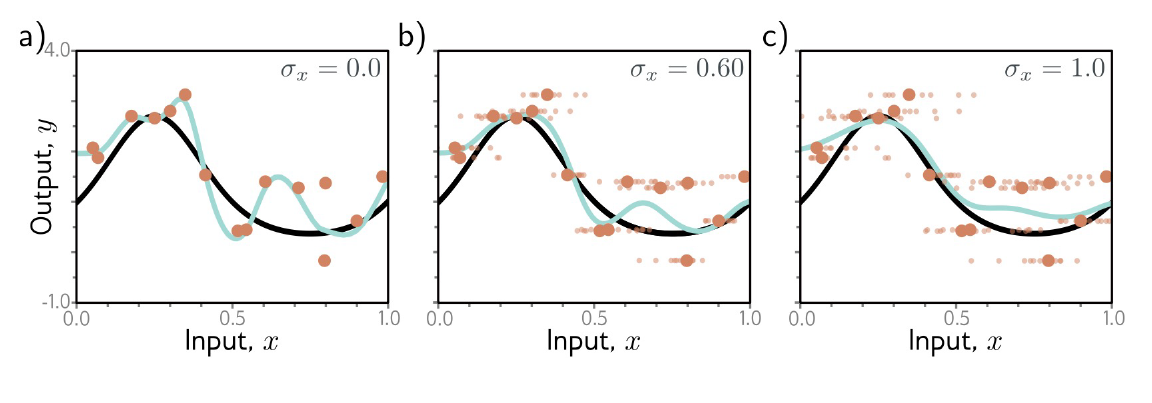
\includegraphics[width=0.8\linewidth]{images/augmentation_noise.png}
        \caption{The effect of adding increasing levels of noise ($\sigma_x$) to the input data during training.}
    \end{figure}
\end{frame}


\end{document}